%% LyX 2.0.2 created this file.  For more info, see http://www.lyx.org/.
%% Do not edit unless you really know what you are doing.
\documentclass[english]{scrbook}
\usepackage{mathptmx}
\usepackage{helvet}
\usepackage{courier}
\usepackage[T1]{fontenc}
\usepackage[latin9]{inputenc}
\usepackage[active]{srcltx}
\usepackage{textcomp}
\usepackage{graphicx}
%\DeclareGraphicsExtensions{.pdf,.png,.jpg}
\makeatletter
%%%%%%%%%%%%%%%%%%%%%%%%%%%%%% Textclass specific LaTeX commands.
\newcommand{\rechead}
    {\centering\normalfont\Large\sffamily\bfseries}

\renewcommand{\subsubsection}
    {\@startsection{subsubsection}{3}{\z@}%
    {-5ex\@plus -1ex \@minus -.2ex}%		
    {1.5ex \@plus .2ex}%
    {\rechead}}

\newcommand{\recipe}[1]{\subsubsection{#1}%
    \hrule height1.75pt width\hsize\vspace*{1\p@}%
    %\hrule height0.25pt width\hsize%
    \nobreak
    \vskip\parskip}
\newcommand{\inghead}[1][]{\large\textbf{Ingredients#1}:}
\newcommand{\ingred}[2][]
    {{\list{}{\rightmargin 2em\leftmargin 2em}%
    \item[]\textit{\inghead[#1]} #2\endlist}}%
%    \hrule height0.25pt width\hsize}
 \renewcommand*\l@subsubsection{\@dottedtocline{3}{3em}{0em}}
 \setlength\parindent{0pt}
 \setlength\parskip{2ex plus 0.5ex}

\makeatother
\setcounter{tocdepth}{4}
\usepackage{babel}
\begin{document}

\title{Memories From My Kitchen}
\date{April 2, 2002}

\author{By Joanne Oeler }

\maketitle



\chapter*{Introduction}

Kitchens are a wonderful place for making memories. My mother was
much happier wielding a needle or a paint brush rather than a spatula,
but I still recall coming in after school to the odor of bread baking
in the oven. And I have a very vivid picture of Mina Love's kitchen
with a big slice of home-cured ham sizzling in the skillet. Like many
of our neighbors, Mina was of Pennsylvania Dutch stock, and firmly
believed that the way to a man's heart is through his stomach. I'm
not sure this applies today, but I've seldom met a man or woman who
did not respond to a well-prepared meal. So, for me, cooking is truly
a labor of love, and the time I spend in the kitchen is often the
best part of my day. My wish for you is that these recipes will make
your time in the kitchen a little easier and a lot more fun.

Most of my recipes are very simple. I'm a big believer in starting
with fresh foods. In Pennsylvania, Mother would send us to the garden
after school to pick the vegetables for supper. You can't get much
fresher than that. I also believe in menu planning and shopping lists,
but having grown up miles from the nearest grocery store and having
lived 19 months in Cleveland (a union town where all stores closed
promptly at 6 p.m.) with only one car, I also believe that some of
your best meals can come from what's on hand if you just have the
courage to try. Know what combinations of herbs and spices you like
and go from there.

A windowsill herb garden is nice and you'll have a hard time using
my recipes without some wine in the house. I can't see buying anything
that is not drinkable so choose a red and a white table wine that
appeal to your taste buds. My standbys are Gallo Hearty Burgundy and
Martini and Rossi Extra Dry Vermouth.

One more hint and it is really as much about relationships as cooking.
My mother-in-law was one of the greatest cooks I've ever known. I
realized early on that I could never match her roast beef or her fabulous
turkey stuffing. And why should I try? After all, I married her \textquotedbl{}Schottzerle\textquotedbl{}
her treasure. I did not want to take away her status as queen of the
kitchen. Visits to her house always brought forth the most perfectly
sliced rare roast beef and my family was generous with their praise.

Mama is gone now and I still can't match her roast beef or her turkey
stuffing but I do not want her recipes to be lost, so I will begin
this cookbook with recipes from Mama's kitchen along with some from
other relatives and friends which are so good that I just stand in
awe. Make that sit in awe -eating of course.

\tableofcontents{}
\chapter{MAMA OELER'S RECIPES}




\recipe{Roast Beef}
\setlength\fboxsep{0pt}
\setlength\fboxrule{0.5pt}
\fbox{
\includegraphics{roast_beef}}

Mama used a Choice eye of round roast. I remember that she cut little
slits in the roast and inserted slivers of garlic. Then she smeared
the top of the roast with a good mustard, seasoned it with salt and
pepper and sprinkled it with freshly chopped parsley. Aunt Rosemary
suggests cooking it in a 325\textdegree{} oven about 30 min. per lb.
Place it in a roasting pan on a rack. Rosemary also suggests putting
a little liquid in the roasting pan. Leslie makes a very good roast
and she uses a meat thermometer . I think this is really safer than
any mathematical formula. One of Mama's secrets was that she could
really carve!! She cooked the beef medium rare -NEVER more, and sliced
it as thinly as possible.


\recipe{Sausage Stuffing}


\setlength\fboxsep{0pt}
\setlength\fboxrule{0.5pt}
\fbox{
\includegraphics{sausage_stuffing}}

For a 12 - 15 lb turkey:


\ingred{1 lb. good quality pork sausage, fried and drained \\
1 small stalk celery with leaves, sliced thinly \\
2 or 3 onions, chopped \\
1/2 lb. fresh mushrooms, sliced \\
1/2 cup parsley, minced \\
1 bag Pepperidge Farms stuffing mix{*} or the equivalent rye bread
\\
1 egg \\
Water or turkey broth to moisten bread}

{*}Rosemary uses the stuffing mix but I remember Mama soaking good
rye bread and then crumbling it into the mixture. (Probably before
the days of stuffing mix). In same pan, in which you have browned
sausage, saut\'{e} the vegetables in 2 or 3 Tbsp. of the drippings. Mix
the vegetables, sausage, bread and egg with sufficient liquid to moisten.
Season to taste with salt, pepper and sage. Stuff turkey.

Optional: I recall Mama put all of her ingredients through an old-fashioned
food grinder and her stuffing had the texture of a pate. You could
get the same result by putting the ingredients in a food processor
before stuffing the bird,


\recipe{Mama's Pot Roast}


\setlength\fboxsep{0pt}
\setlength\fboxrule{0.5pt}
\fbox{
\includegraphics{pot_roast}}


\ingred{5 lb. boneless beef rump roast (she used tenderizer on this) \\
1/3 cup flour \\
2 Tbsp. oil Accent, salt and pepper \\
3 Tbsp wine vinegar \\
Pinch celery seed \\
1/8 tsp. oregano \\
1 onion, sliced \\
2 cups whole small white onions \\
8 small carrots; pared \\
3 Tbsp. flour \\
1/2 cup water}

1 Roll beef in 1/3 cup flour to coat on all sides. In Dutch Oven,
brown over med. heat 15 - 20 min. Sprinkle with Accent, salt and pepper
as you turn it. 2. Add celery seeds, oregano, vinegar and sliced onion.
Cover tightly. Simmer turning occasionally 2 3/4 - 3 1/2 hrs 3. Add
the vegetables, tucking them around the roast. Simmer until the beef
is fork tender and vegetables are done. 4. Remove the meat and vegetables
to a warm platter. Add sufficient water to Dutch Oven to make 2 1/2
cups liquid. Mix flour with 1/2 cup water and stir into liquid to
thicken gravy.


\recipe{Mama's Pfeffern\"usse}


\setlength\fboxsep{0pt}
\setlength\fboxrule{0.5pt}
\fbox{
\includegraphics{pfeffernusse}}


\ingred{3 cups sifted all-purpose flour \\
3/4 tsp. ea. baking soda, baking powder, salt, mace, ground allspice,
ground cardamom \\
1/4 tsp. ground black pepper \\
1/4 tsp. anise seeds \\
1 cup honey \\
3 Tbsp. shortening \\
1 egg}

Re-sift flour with next 8 ingredients. Heat honey until hot but do
not boil. Add shortening to honey, let cool. Beat in egg. Stir in
dry ingredients, being careful not to over-mix. Let dough stand 10
min. to stiffen for easy handling. Shape into 1\textquotedbl{} balls.
Place on lightly greased baking sheet. Bake 10 - 15 min. at 350\textdegree{}.
Cool and frost.


\ingred{for Frosting: \\
1 egg white, unbeaten \\
2 Tbsp. honey \\
1/4 tsp. ground anise seed \\
1 1/2 cups sifted confectioners sugar}

Combine first 3 ingredients in mixing bowl. Gradually beat in confectioners
sugar with electric mixer. Beat thoroughly. Place 12 - 14 cookies in
a bowl. Add 2 Tbsp. frosting. Stir to coat all sides. Lift out with
a fork onto wire rack. I.et frosting harden. Makes about 50 cookies.
May be stored in a tin box or cookie jar.


\recipe{Hard Lebkuchen}


\setlength\fboxsep{0pt}
\setlength\fboxrule{0.5pt}
\fbox{
\includegraphics{lebkuchen}}


\ingred{2 eggs, lightly beaten \\
4 Tbsp. honey \\
2 cups sugar \\
1 tsp. cinnamon \\
1/4 tsp. ginger \\
1/16 tsp. ea. pepper, cloves, nutmeg \\
4 Tbsp. cocoa \\
1/2 lemon, rind grated plus juice \\
3 1/4 cups sifted all-purpose flour \\
1/2 tsp. soda \\
1/4 tsp. cardamom \\
10 Tbsp. ground hazelnuts (may substitute)}

Mix all ingredients thoroughly. Mixture will be very crumbly. Pat
onto a cookie sheet with a spoon. Bake at 300\textdegree{} 15 - 20
min. Remove from oven and while still warm, cut into diamond shapes.
Glaze with a mixture of 2 cups confectioners sugar and the juice of
1 lemon.


\recipe{Anise Drop Cookies}


\setlength\fboxsep{0pt}
\setlength\fboxrule{0.5pt}
\fbox{
\includegraphics{anise}}



\ingred{3 eggs, beaten until light \\
3 cups light brown sugar \\
2 Tbsp. anise seeds \\
1 tsp. salt \\
1 tsp. baking soda dissolved in 2 Tbsp. hot water \\
4 1/2 cups flour}

Add sugar to eggs, beating continuously until light. Add seeds, salt
and soda. Mix in flour. Form hickory nut sized balls. Roll in granulated
sugar and place on greased cookie sheet. Bake 10 min. in 350\textdegree{}
oven. Allow to remain on cookie sheet until cool. These improve with
age.


\recipe{Mama's Gugelhopf}

\setlength\fboxsep{0pt}
\setlength\fboxrule{0.5pt}
\fbox{
\includegraphics{gugelhopf}}

\ingred{1/4 lb. sweet butter \\
1 cup sugar \\
3 eggs \\
Grated rind of 1 lemon \\
2 cup sifted flour \\
1 tsp. baking powder \\
3/4 tsp. baking soda \\
1 cup sour cream {*} \\
1 cup raisins or currants, dredged in flour \\
1 tsp. vanilla \\
1/2 tsp. almond extract}

Cream butter and sugar. Beat in eggs, one at a time. Sift flour with
baking powder and soda; add alternately with sour cream. Add raisins
and flavorings. Pour into a greased Bundt cake pan. Bake at 350\textdegree{}
for 30 - 40 min. or until tester comes out clean. Let stand 10 min.
on wire rack before removing from pan. If difficult to remove, place
a damp towel over the pan. May be glazed with the same glaze as the
lebkuchen.

{*}Mama omitted the amount of sour cream from the recipe she sent
me so I'm guessing. The batter should be the consistency of a layer
cake mix.


\recipe{Aunt Gerry's Lemon Pie}

\setlength\fboxsep{0pt}
\setlength\fboxrule{0.5pt}
\fbox{
\includegraphics{lemon_pie}}

\ingred{1 recipe favorite pastry or 1/2 pkg. mix \\
2 1/4 cups sugar \\
4 Tbsp. cornstarch \\
4 Tbsp. flour \\
1/4 tsp. salt \\
2 cups water \\
4 eggs, separated\\
 1 Tbsp. grated lemon rind \\
6 Tbsp. fresh lemon juice\\
 2 Tbsp. butter \\
1/4 tsp. lemon extract}
\begin{enumerate}
\item Roll out the pastry to a 12\textquotedbl{} round. Fit into a 9\textquotedbl{}
pie plate and trim the overhang to 1/2'' turn under the overhang,
flush with rim. Flute to make a high stand-up edge and prick all over
with a fork. Bake in a 425\textdegree{} oven until golden (about 15
min.). Cool completely on wire rack. 
\item Mix 1 3/4 cups of the sugar, cornstarch, flour and salt in a medium
sized bowl. 
\item Heat the water to boiling in a medium sized saucepan, Lower heat to
medium and slowly add the sugar mixture, stirring constantly. Cook
5 to 7 minutes or until mixture holds a line when cut with a spoon.
Do not let boil. Remove from heat. 
\item Beat the egg yolks slightly in a small bowl. Stir in 1/2 cup of the
hot mixture then quickly stir this into the mixture in saucepan. Return
to med. heat and cook, stirring constantly 3 min or until mixture
thickens and mounds softly. Remove from heat. 
\item Stir in lemon rind, juice and butter until completely blended. Pour
into shell. 
\item Beat egg whites with lemon extract until foamy and double in volume.
Sprinkle remaining 1/2 cup sugar over whites 1 Tbsp. at a time, beating
constantly until sugar is completely dissolved and stiff peaks form. 
\item Pile meringue onto hot filling being sure to spread to edge of crust.
\item Bake in 350\textdegree{} oven 12 min. or until meringue is golden
brown. Cool completely on wire rack.
\end{enumerate}
This is just the best lemon pie you'll ever eat!

I'll never forget the first time I tasted Pecan Pie. It was in 1941
on our first trip from Pennsylvania to Florida. I thought I'd died
and gone to heaven. Jan Willis makes one that duplicates that experience.


\recipe{Jan's Pecan Pie}

\setlength\fboxsep{0pt}
\setlength\fboxrule{0.5pt}
\fbox{
\includegraphics{pecan_pie}}


\ingred{1 recipe pastry prepared as for Lemon Pie but left unbaked \\
3 eggs \\
1 cup Dark Karo syrup \\
1 cup pecan halves 1 tsp. vanilla \\
1 cup sugar \\
1/2 cup melted butter \\
1/4 tsp. salt}

Beat eggs until light. Add sugar and beat again. Add butter, Karo,
salt and vanilla. Mix well. Pour into unbaked pie shell and bake 45
min in preheated 350\textdegree{} oven. Custard should be set. Test
with knife. It should come out clean. 


\chapter{MISCELLANEOUS}


\recipe{Kahlua}
\setlength\fboxsep{0pt}
\setlength\fboxrule{0.5pt}
\fbox{
\includegraphics{kahlua}}



\ingred{2 oz. instant coffee\\
 4 cups sugar \\
2 cups boiling water \\
1 pt. vodka \\
1 vanilla bean}

Dissolve coffee and sugar in boiling water. Be sure to dissolve completely.
Let cool. Add vodka. Pour into two sterilized bottles. Add 1/2 vanilla
bean to each bottle. Let age at least 30 days. Mary Hamilton gave
me this recipe and I prefer it to the original. I think it's the vanilla
bean.


\recipe{Instant Russian Tea}

\setlength\fboxsep{0pt}
\setlength\fboxrule{0.5pt}
\fbox{
\includegraphics{russian_tea}}


\ingred{1 cup sugar \\
3/4 cup Tang \\
1/3 cup instant tea \\
1/2 tsp. cinnamon \\
1/2 tsp. cloves \\
1/2 small pkg. lemonade mix}

Mix all together. Store in tightly covered jar. Stir 1 - 2 tsp. into
cup of boiling water for each serving.

Our family likes curry and I am so disappointed with the quality of
store-bought chutney that I make this up when cranberries are in season.


\recipe{Cranberry Chutney}

\setlength\fboxsep{0pt}
\setlength\fboxrule{0.5pt}
\fbox{
\includegraphics{cranberry_chutney}}


\ingred{1 lb. fresh cranberries \\
1 cup seedless raisins \\
1 2/3 cup sugar \\
1 Tbsp ground cinnamon\\
 1 1/2 tsp. ground ginger \\
1/4 tsp ground cloves \\
1 cup water \\
1/2 cup chopped onion \\
1 medium-sized apple, pared, cored and chopped \\
1/4 cup chopped almonds}

Combine cranberries, raisins, spices and water in a large saucepan.
Bring to a boil and cook 15 min. or until berries pop and mixture
thickens. Stir in onion, apple and nuts. Simmer 15 min. more. Mixture
should be thick. Pour into sterilized jars. Store in refrigerator.
Makes 4 cups.


\recipe{Beet-Cabbage Relish}

\setlength\fboxsep{0pt}
\setlength\fboxrule{0.5pt}
\fbox{
\includegraphics{beet_relish}}


\ingred{2 - 16 oz. cans beets, chopped \\
4 cups cabbage, chopped \\
4 oz. horseradish \\
1 cup sugar \\
3/4 cup light corn syrup \\
1 tsp. salt \\
1/8 tsp. pepper \\
1 cup white vinegar\\
 1 cup water}

Combine first seven ingredients. Bring the vinegar and water to a
boil. Pour over the vegetables. Put in hot, sterilized jars. Store
in refrigerator.

Note: Both the chutney and the relish could be processed in a hot
water bath. Then you would not need to store them in the refrigerator.
I'm lucky enough to have lots of refrigerator space and prefer foods
that have not been \textquotedbl{}canned\textquotedbl{}.

My family thinks that Pesto is one of the all-time great culinary
inventions. It's wonderful on hot pasta, rice or stirred into saut\'{e}ed
shredded zucchini Put a few Tablespoons full into a canned soup such
as Minestrone or spread on fresh halves of tomatoes and bake. John
likes chicken marinated in Pesto and broiled. You can vary the amounts
of basil and parsley to suit your taste. This recipe is our favorite.


\recipe{Pesto}

\setlength\fboxsep{0pt}
\setlength\fboxrule{0.5pt}
\fbox{
\includegraphics{pesto}}


\ingred{4 cups fresh basil leaves \\
3 cloves garlic \\
1/2 - 1 cup fresh parsley(not cilantro) \\
1/2 cup olive oil \\
1/2 tsp. salt\\
 1/2 cup pine nuts{*}\\
 1/2 cup good Italian cheese (we like Pecarino){*}}

With food processor running, drop in 3 cloves garlic. When finely
minced, add the basil and parsley and salt. Process until somewhat
chopped; then add olive oil in a stream through top. Add more oil
if necessary to make a smooth paste. IF you are going to use the pesto
soon, add the nuts and cheese. {*}IF you are going to freeze it, omit
these two ingredients. It keeps well in the refrigerator in an airtight
container with l/2\textquotedbl{} olive oil on top. Freeze in 1/2
cup batches-sufficient for 4 servings of pasta. You just dilute the
pesto with 2 Tbsp. of the hot water in. which you cooked the pasta,
toss and serve.

For those of you unfamiliar with the gourmet qualities of the humble
grits I dug out this recipe which is one of my favorites.


\recipe{Cheese Grits}

\setlength\fboxsep{0pt}
\setlength\fboxrule{0.5pt}
\fbox{
\includegraphics{cheese_grits}}


\ingred{1 cup quick grits, cooked as pkg. directs \\
1/4 lb. butter or margarine \\
6 oz good cheddar \\
1/2 cup milk, blended into 2 beaten eggs}

Add butter and cheese to hot grits, then add egg/milk mixture. If
the grits are very hot, stir 1/2 cup full of hot mixture into egg/milk
mixture and then stir all into grits Blend all ingredients well. Turn
into an oven-proof greased casserole and bake at 350\textdegree{}
for 45 min. Knife should come out clean.


\recipe{Pilaf}

\setlength\fboxsep{0pt}
\setlength\fboxrule{0.5pt}
\fbox{
\includegraphics{pilaf}}

\ingred{1 egg, stirred into 1 cup medium buckwheat groats (kasha)\\
 3 Tbsp oil \\
1 medium onion, chopped \\
3 1/2 cups boiling water \\
1/2 cup long grain rice (not instant) \\
2 bouillon cubes 1 cup frozen peas}

In a large skillet, cook onion in oil until tender. Add kasha mixture
and cook until the grains are dry and separated, stirring constantly.
Slowly add boiling water, bouillon, and if you like, 1/2 tsp. salt.
(I think the bouillon cubes give enough salt). Reduce heat to low.
Cover and simmer 15 min. Add peas and cook 5 min more until liquid
is absorbed. Serves 12. This pilaf goes well with Middle Eastern dishes
such as the Greek Stew.

One of Leslie's favorites is Pickled Okra. This recipe is from the
LBJ Ranch.


\recipe{Pickled Okra}

\setlength\fboxsep{0pt}
\setlength\fboxrule{0.5pt}
\fbox{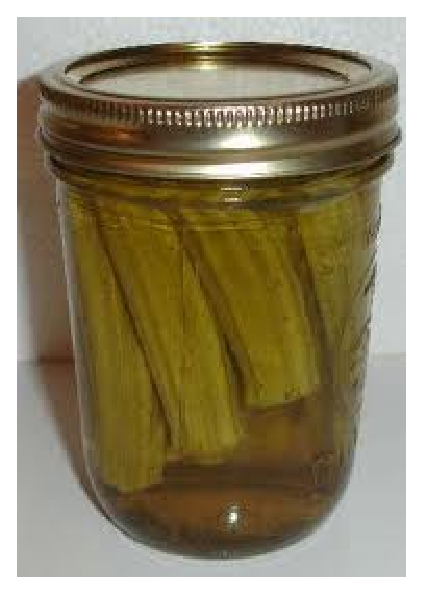
\includegraphics{okrapickled}}

\ingred{2 tsp. dill seed \\
2 pkg. (10 oz.) frozen okra or the equivalent of fresh\\
 2 dried red peppers \\
2 canned chili peppers \\
4 cloves garlic, peeled \\
1 1/4 cups white vinegar \\
3 Tbsp. salt}

If using frozen okra, thaw and drain. Sterilize 2 pint jars and lids
and keep in hot water while preparing recipe. In small saucepan, combine
vinegar, salt and 1/2 cup water. Bring to boiling. Place 1/2 tsp.
dill seed in bottom of each jar. Pack okra into jars being careful
not to break pods. On top of okra, put 1/2 tsp. dill seed, 1 red pepper,
1 chili pepper and 2 cloves garlic. Pour the hot vinegar mixture over
the top of each jar. Cap according to manufacturer's directions. Let
stand at room temperature until completely cooled. Refrigerate at
least 2 weeks before serving to let flavors develop. Serve chilled
with a real Texas meal such as Barbecued Brisket and Beans.


\chapter{APPETIZERS}


\recipe{BBQ Pecans}

\setlength\fboxsep{0pt}
\setlength\fboxrule{0.5pt}
\fbox{
\includegraphics{bbqpecans}}
\ingred{1 Tbsp. sugar\\
 2 Tbsp, cider vinegar\\
 2 cups pecan halves\\
 1 tsp. margarine \\
1/2 tsp. seasoned salt.}

Mix sugar and vinegar in container with cover. When sugar is dissolved,
add pecans and shake until nuts are thoroughly coated. Spray a shallow
baking pan with Pam and place nuts in pan in 250\textdegree{} oven.
Bake until lightly brown, stirring often. Add margarine and seasoned
salt and stir to coat nuts. Continue baking until a nice brown color.
Cool and store in a tightly covered container or in the fridge. This recipe
makes 2 cups so I usually double it and bake in my roaster pan.


\recipe{Ceviche}
\setlength\fboxsep{0pt}
\setlength\fboxrule{0.5pt}
\fbox{
\includegraphics{ceviche}}

\ingred{1 lb. fresh fish fillets (or shrimp or scallops) \\
juice of 20-30 Mexican limes \\
1 medium onion, finely chopped \\
2 medium tomatoes, chopped \\
1 medium green pepper, finely chopped \\
30 pitted green olives \\
1/8 tsp. comino \\
20 capers \\
1/4 cup olive oil\\
 Salt, pepper to taste\\
 1 Tbsp. parsley, chopped \\
1 tsp. oregano}

Cut seafood into dime-size pieces and marinate in lime juice in a
glass bowl for 4 to 5 hours at room temp. Drain well, mix with other
ingredients and serve ice cold.


\recipe{Cheese cookies}

\setlength\fboxsep{0pt}
\setlength\fboxrule{0.5pt}
\fbox{
\includegraphics{cheesecookies}}
\ingred{1/4 lb. butter or margarine \\
1/2 cup New York State sharp cheese\\
1 1/2 cup sifted flour \\
1 tsp. salt\\
 1 tsp. white pepper\\
 1 tsp. hot sauce \\
1/2 cup chopped pecans (optional)}

Grate cheese and mix with other ingredients. Form into roll and wrap
in plastic wrap. Chill or freeze. Slice and bake in 250\textdegree{}
oven on greased cookie sheet till nicely browned. Don't slice more
than 1/2\textquotedbl{} thick.


\recipe{Hot Broccoli Dip}

\setlength\fboxsep{0pt}
\setlength\fboxrule{0.5pt}
\fbox{
\includegraphics{hbd}}
\ingred{3 stalks celery, chopped fine \\
1/2 onion, chopped fine \\
1 small can of mushroom pieces}

Saut\'{e} above ingredients in margarine until limp. Add one roll garlic
process cheese and 1 can mushroom soup. Stir till cheese is melted.
Cook 1 pkg. chopped broccoli according to directions; drain and combine
with above. Serve in a chafing dish with Fritos or other sturdy crackers.
This dip was all the rage at our parties in the 60s, but I love it
still, maybe because I love anything with cheese and/ or broccoli.

The next recipe comes from Katina Xeros, the wife of the Richardson
Symphony conductor. She taught me to make these wonderful dolmas for
a Greek Dinner Party I gave to benefit the Dallas Metropolitan Ballet
Co.


\recipe{Katina's Dolmas}
\setlength\fboxsep{0pt}
\setlength\fboxrule{0.5pt}
\fbox{
\includegraphics{dolma}}

\ingred{1 pint jar grapevine leaves \\
1 medium onion, grated \\
1/4 lb. good margarine \\
1 1/2 lb. lean ground beef \\
1/2 cup long grain rice \\
1 1/2 tsp. salt Pepper to taste \\
1 Tbsp. tomato paste {*} \\
2 Tbsp. each chopped mint and parsley\\
 Juice of 1 lemon}

Rinse grapevine leaves in running cold water once or twice, depending
on how salty you want your dolmas to be. Let rinsed leaves stand in
warm water as you prepare meat mixture. Saut\'{e} onion in 1/4 stick
of oleo until golden; add tomato paste. Add this mixture to ground
beef and remaining ingredients except butter and lemon juice. This
mixture needs to be soft so dig in with your hands adding 3 or 4 Tbsp.
of water to soften. Place 1 tsp. of meat mixture in the center of
one grapevine leaf (on veined side). Turn over piece of leaf nearest
you, then sides and roll up into narrow roll. Arrange dolmas, in a
deep sauce pan which you will have lined with several leaves. (Use
the ones which are torn and unsuitable for the rolls). Place the dolmas
in layers with the seamed side down. Cover with a few more leaves.
Add remaining margarine, 2 cups water, and lemon juice. Cover and
cook slowly for one to one and one half hours. Serve plain or with
sour cream or the Aveglemono Sauce. (recipe with sauces)

{*}If you don't have fresh mint, use 1 tsp. of the dried.


\recipe{Liptauer}
\setlength\fboxsep{0pt}
\setlength\fboxrule{0.5pt}
\fbox{
\includegraphics{liptauer}}

\ingred{8 oz. cream cheese \\
1/4 lb. butter or good margarine \\
1 Tbsp. caraway seed, crushed in mortar\\
 1 Tbsp. capers, minced \\
1 Tbsp. chives or green onion tops, minced\\
 1 Tbsp. dry mustard \\
1 anchovy, minced.}

Blend all ingredients and form into ball. Sprinkle with paprika and
chill. Serve with party rye or vegetables.

This was another recipe I developed for an ethnic benefit dinner. It
is Czech in origin and definitely not a cheese ball for the faint
hearted. It has a unique, hearty flavor.


\recipe{Piping Pigs}

\setlength\fboxsep{0pt}
\setlength\fboxrule{0.5pt}
\fbox{
\includegraphics{pipingpig}}
\ingred{1 pkg. wieners \\
1 cup prepared salad mustard\\
1 cup red currant jelly}

Cut wieners into bite size pieces. Put in 1 1/2 qt. oven casserole.
Mix mustard and jelly together and pour over cut up wieners. Put in
oven at 300\textdegree{} and cook till bubbly hot, - about 20 min.
Put in chafing dish and serve with toothpicks. Tastes exotic but it's
so easy.

The next recipe came from another Ballet function but this one was
an after-performance Buffet for Natalia Makarova the first time she
danced in Dallas. I remember thinking she was incredibly tiny and
oh, so shy.


\recipe{Water Chestnut Meatballs}

\setlength\fboxsep{0pt}
\setlength\fboxrule{0.5pt}
\fbox{
\includegraphics{wcmeatballs}}
\ingred{2 cups soft bread crumbs \\
1/2 cup milk \\
1 Tbsp. soy sauce\\
 1/2 tsp. garlic salt \\
1/4 tsp. onion powder\\
 1/2 lb. ground beef 1/2 lb. ground pork \\
1 - 5 or 6 oz. can water chestnuts, drained and finely chopped.}

Combine bread crumbs, milk, soy sauce, garlic salt and onion powder.
Add ground beef and pork and water chestnuts. Mix well. Form meat
mixture into 1\textquotedbl{} balls; place on 15 1/2 x 10 1/2 baking
pan. Bake at 350 for 18 - 20 min. Makes 5 doz. Serve hot from chafing
dish with toothpicks. Personally, I like them plain but you might
want to serve them with a teriyaki or sweet/sour sauce.


\recipe{Make Ahead Quiche}

\setlength\fboxsep{0pt}
\setlength\fboxrule{0.5pt}
\fbox{
\includegraphics{quiche}}

\ingred{One 8\textquotedbl{} pie shell \\
2 cups chopped green onions\\
 1 Tbsp. butter \\
1 egg, beaten\\
 1/2 cup milk \\
1 - 8 oz. pkg. cream cheese\\
 1/4 tsp. Worcestershire Sauce \\
1/2 tsp. salt Paprika to taste}

Saut\'{e} onions in butter until soft. In a separate pan, mix egg, milk,
cream cheese and seasonings. Heat over med. heat, stirring with a
whisk until smooth and creamy. Spread onions over bottom of pie shell;
pour over cheese mixture{*}. Bake at 350\textdegree{} until a knife
can be inserted and come out clean, - about 35 min. {*} Can be covered
with foil and refrigerated overnight.


\recipe{Oysters A La Kaphan's}

Kaphan's is our favorite restaurant in Houston and the manager circulates
through the restaurant during mealtimes offering these wonderful hors
d'oeuvres hot from the pan. My version follows:
\setlength\fboxsep{0pt}
\setlength\fboxrule{0.5pt}
\fbox{
\includegraphics{kaphans}}

Salt and pepper 24 medium to large oysters and dredge in flour. Saut\'{e}
in a heavy skillet on top of stove until crisp and browned on both
sides.

In the meantime, place in a saucepan: 2 Tbsp. melted butter 1 cup
A-l steak sauce 2 Tbsp. Worcestershire sauce 2 jiggers dry sherry
wine

Heat over low fire until thoroughly heated. Do not boil. Blend 2 Tbsp.
water and 3 Tbsp. flour. Stir into sauce. Place saut\'{e}ed oysters on
a hot serving plate and pour sauce over. Insert cocktail picks and
serve hot. (Sauce can be strained, reheated and used again.)


\recipe{Sausage Balls}


\ingred{1 lb. sharp cheddar cheese \\
1 lb. sausage \\
2 cups Bisquick}

Mix and roll into balls the size of a large walnut. Bake in a 450\textdegree{}
oven for 15 min. Serve hot.


\recipe{Tamale Balls}

\setlength\fboxsep{0pt}
\setlength\fboxrule{0.5pt}
\fbox{
\includegraphics{tamaleballs}}
\ingred{1 lb. ground beef \\
1 lb. ground pork \\
1 Tbsp. chili powder \\
1 1/2 cups corn meal \\
2 tsp. salt \\
3/4 cup tomato juice \\
4 med. cloves garlic}

Mix beef and pork together. Add all other ingredients. Mix well with
hands and form into small balls the size of large marbles. Place in
sauce (recipe follows) and simmer about 2 hrs. Keep hot in chafing
dish. Serve on tooth picks. 


\ingred{Sauce\\
 2 large cans tomatoes\\
 2 tsp. salt \\
1 Tbsp. chili powder}

Mash tomatoes (or puree coarsely in food processor. Simmer all ingredients
2 hrs.


\recipe{Tuna Pate}

\setlength\fboxsep{0pt}
\setlength\fboxrule{0.5pt}
\fbox{
\includegraphics{tunapate}}
\ingred{2 pkg. (8 oz.) cream cheese at room temp. \\
3 cans oil packed tuna \\
4 tsp. lemon juice \\
4 tsp. grated onion \\
2 Tbsp. capers, drained \\
1/2 cup finely chopped walnuts \\
Salt and pepper to taste\\
 1 1/2 tsp. dry mustard \\
1/2 tsp. dry thyme}

Drain tuna well and mix with softened cream cheese. Stir in remaining
ingredients and shape into ball or mold into appropriate shape. Decorate
with chopped parsley and serve with Melba toast.


\chapter{SOUPS}


\recipe{Old Fashioned Bean Soup}
\setlength\fboxsep{0pt}
\setlength\fboxrule{0.5pt}
\fbox{
\includegraphics{beansoup}}

Pick over and rinse 1 lb. Great Northern beans. Place in large soup
pot and cover with cold water. Place over high heat and bring to a
boil. Add 2 tsp. baking soda and boil for 60-90 seconds. Drain and
rinse well. Return to pot and cover well with water (at least 8 cups).
Add 1 meaty ham bone. Bring to boiling, reduce heat, cover and simmer
for 2 - 4 hrs. until beans are tender. Add 1 large chopped onion,
1 bay leaf and 1/2 tsp.pepper. Taste for salt. If too salty, add 1
pared diced potato. (This will aid any soup which is too salty.) Cook
1 hr. more or until beans are very tender. Remove bay leaf and ham
bone. Cut meat from bone, return to pot and serve.

Note: The preboiling with baking soda is supposed to relieve the gassy
aftereffects of eating beans. Sometimes it works and sometimes it
doesn't, but I recommend it for all my soup recipes.

When John was in the Air Force, he was stationed at McDill Field in
Tampa, Fla. After we were married, he took me there for a visit and
we ate at a wonderful Cuban restaurant called Las Novedades. This
is one of my favorites from there


\recipe{Garbanzo Bean Soup}

\setlength\fboxsep{0pt}
\setlength\fboxrule{0.5pt}
\fbox{
\includegraphics{garbonzo}}
\ingred{3/4 lb. garbanzo beans (chick peas) \\
1 onion \\
1 beef bone \\
1 chorizo sausage(very spicy hot sausage) \\
1 pinch saffron \\
1 1/2 qts. water \\
1/2 lb. potatoes \\
1/4 lb. salt pork or bacon \\
1 ham bone \\
2 oz. lard or oil (optional) \\
1 Tbsp. salt}

Soak garbanzos overnight in sufficient water to cover bean. Drain
and precook with baking soda. Drain and rinse. Return to pot with
water and both bones. Simmer 45 min. Fry bacon and onions in lard
or oil; add to pot with potatoes, saffron and salt. When potatoes
and beans are done, remove from fire. Remove bones and cut meat from
them. Add thinly sliced chorizo, and serve with crusty bread.


\recipe{Black Bean Soup}


\ingred{1/2 lb. black beans \\
1 cup olive oil \\
1 large onion, chopped \\
1 clove garlic \\
 Tbsp. salt \\
1 oz. salt pork or bacon \\
1/4 lb. ham bone\\
 1/2 cup vinegar\\
 3 green peppers, chopped \\
3 bay leaves\\
 1 1/2 quarts water}

Soak beans thoroughly. Fry onion, green pepper and garlic in 1/2 cup
oil. Combine all ingredients except vinegar and cook over low heat
until beans are tender and the liquid is thick. Add vinegar just before
serving. I usually serve the vinegar separately and let each person
add it to his taste.


\recipe{Red Gazpacho}

\setlength\fboxsep{0pt}
\setlength\fboxrule{0.5pt}
\fbox{
\includegraphics{gazpacho}}
\ingred{3 cups fresh tomatoes, peeled and coarsely chopped\\
 1 1/2 cups cucumbers, peeled and chopped \\
1 green pepper, cored, seeded and coarsely chopped \\
1 clove garlic, crushed \\
1/2 cup water \\
5 Tbsp. olive oil 1\\
/4 cup red wine vinegar Salt to taste \\
2 slices fresh bread, cubed}

Combine all ingredients in the container of a blender or food processor
and blend at high speed until ingredients are smooth. Taste, and
adjust salt and vinegar to taste. Chill before serving.


\recipe{White Gazpacho}


\ingred{3 medium cucumbers, peeled and cut into chunks \\
3 cups cooled chicken broth \\
3 cups sour cream or yogurt \\
3 Tbsp. white vinegar \\
1 1/2 tsp. salt \\
1 clove garlic, crushed \\
2 tomatoes chopped 1\\
1/2 cup sliced green onions\\
 1/2 cup finely chopped parsley\\
 1/2 cup sliced almonds, toasted (optional)}

Whirl cucumbers in blender or food processor with a little chicken
broth until smooth. Stir in remaining broth, sour cream, vinegar,
salt and garlic. Stir gently and chill. When ready to serve, sprinkle
tomatoes, onions, parsley and almonds on top as a garnish.

These soups are so easy and delicious when the vegetables are in season.
I just keep them in refrigerator for quick refreshing snack.


\recipe{Cheese Mushroom Soup}

This soup was served at the First Epiphany Bazaar and has been a family
favorite ever since. It is much easier if you have a food processor.
Just chop and shred and slice in the order given in the recipe You
don't even have to wash the processor between ingredients.


\ingred{6 Tbsp. margarine \\
1 small onion, chopped \\
1/2 lb. mushrooms, sliced \\
4 Tbsp. flour \\
3/4 tsp. dry mustard \\
2 beef bouillon cubes dissolved in 2 cups water \\
2 cups milk \\
 2 cups medium cheddar, shredded \\
1 carrot shredded\\
 3 Tbsp. fresh parsley, minced \\
Salt and pepper to taste}

Melt margarine in a 4-qt. pan set over med. heat. Add onions and mushrooms.
Cook, stirring occasionally until onion is limp and mushroom liquid
evaporates. Stir together the flour and mustard; stir into mushrooms.
Gradually stir in bouillon. Bring to a boil, stirring until thickened.
Remove from heat and stir in milk. If making ahead, cover and chill
at this point. Before serving, reheat, remove from heat, and stir
in cheese until melted. Season to taste. Garnish with shredded carrot
and parsley.

We picked up our Cioppino recipe while living in San Diego, California.
One of the stories told about Cioppino, is that it was made at the
end of the day when the fishermen came in and everyone \textquotedbl{}Chipped
into the pot\textquotedbl{} with their unsaleable fish.


\recipe{Cioppino}

\setlength\fboxsep{0pt}
\setlength\fboxrule{0.5pt}
\fbox{
\includegraphics{cioppino}}
\ingred{1 1/2 lb. any firm-fleshed fish such as sea bass, rock fish or snapper\\
1 lb. raw shrimp \\
1 large crab (optional) \\
1 doz. clams or 1 can minced clams \\
1/2 cup olive oil (I use 3/8 cup olive oil and 1/8 cup salad oil)
\\
1 large clove garlic, minced\\
 1 1/2 cups onion, chopped \\
1 cup green pepper, chopped \\
1 - 8 oz. can tomato sauce \\
1 No. 2 1/2 can red tomatoes\\
 2 cups red table wine (Gallo Hearty Burg) \\
1/2 cup minced parsley \\
1 tsp. salt \\
1/4 tsp. freshly ground black. pepper\\
 1/2 tsp. oregano, crumbled\\
 1/4 tsp. basil, crumbled}

Cut the fish into serving sized pieces. Shell shrimp and devein. Clean
and crack the crab saving all large pieces of shell with meat in them.
Scrub clams. Cook the onion and garlic and green pepper in hot oil.
Add the tomato sauce, tomatoes, wine and parsley. Add the seasonings.
Cook for 30 min. Arrange the fish, crab and shrimp in layers in a
large Dutch Oven. Pour the sauce over the seafood and cook over low
heat until the fish is tender, about 30 min. Watch closely as less
firm fish will cook more quickly. Add the clams and when they open,
sprinkle with additional parsley and serve. If you are lucky enough
to have seafood in the shell, you may want to offer bibs with this
dish. If you add a tossed salad and French bread you have a fabulous
meal.


\recipe{Lentil Soup}


\ingred{2 cups dried lentils \\
3 onions, chopped\\
 2 carrots, diced \\
2 quarts water \\
2 - 8 oz. cans tomato sauce \\
1 bay leaf 1 1/2 tsp. salt \\
1 ham hock\\
 1 cup dry red wine (Gallo H.B. again)\\
 1 lb. Italian sausage links or other garlicky sausage}

Wash and drain lentils. Place in a 6 to 8 qt. Dutch Oven. Add onions,
carrots, water, tomato sauce, bay leaf and salt. Bring to a boil.
Add ham hock and wine. Cover and simmer until ham is tender (about
2 1/2 hrs.) Remove bones and fat from ham. Return to pot with sausages
and simmer 30 min. or until sausages are done. Remove sausages and
slice. Return to soup and serve 6 very heartily.

I searched for years for a good minestrone recipe and I think this
one is it. It is the blend of seasonings which makes it so good so
don't leave out any of the herbs.


\recipe{Minestrone}


\ingred{1 cup Great Northern beans\\
 4 cups water\\
 3 Tbsp. oil (part olive oil)\\
 2 cups finely chopped onion\\
 2 large cloves garlic, minced \\
1 1/2 cups leeks, finely shredded\\
 2 cups cabbage, finely shredded\\
 1 lb. carrots, finely diced\\
2 cups zucchini, quartered and sliced \\
2 large tomatoes, peeled and cubed \\
1/2 cup Parsley, finely chopped \\
1/4 cup fresh basil, finely chopped or 1 Tbsp. dried basil\\
 1 tsp. fresh rosemary, finely chopped or 1/2 tsp. dried \\
1/8 tsp. powdered cloves \\
4 cups beef bouillon (made with cubes)\\
 3/4 cup small elbow macaroni}

Soak beans overnight. Drain and put in a large pot and add 4 cups
of water. Bring to a boil, covered and simmer for about an hour or
until beans are tender. Drain; save 2 cups of the liquid. In a large
Dutch Oven, heat the oil. Add the onion and cook, stirring until wilted.
Add the leeks, cabbage, carrots, zucchini and tomatoes. Cook, stirring
occasionally about 10 min. Add the parsley, herbs and the reserved
bean liquid and the bouillon. Put half the beans in the food processor
and puree. Add to the soup. Add the remaining beans. Bring to a boil
and simmer for 30 min. Add the macaroni and cook until tender - about
15 min. Serve sprinkled with parsley and pass the Parmesan Cheese.

I grew up thinking that Borscht was that pink stuff in jars at the
deli. But Leslie introduced me to Russian food at the Russian Tea
Room in N.Y.C. and the search was on for a good Borscht recipe. This
one is supposed to be a favorite of Rudolf Nuryev's.


\recipe{Borscht a la Nuryev}

\setlength\fboxsep{0pt}
\setlength\fboxrule{0.5pt}
\fbox{
\includegraphics{borscht}}
\ingred{2 1/2 lb. boneless beef chuck \\
2 soup bones\\
 2 onions, halved \\
1 small clove garlic \\
1 Tbsp. salt \\
1/2 Tbsp. pepper \\
8 cups water \\
3 carrots, sliced\\
 1 - 16 oz. can tomatoes\\
1 bay leaf 3 med. beets, peeled and sliced\\
 1 small head cabbage, shredded \\
3 med. potatoes, peeled and sliced}

Place chuck, bones, onion, garlic, salt and pepper and water in a
large soup pot. Cover and bring to a boil. Skim off film. Cover and
simmer 30 min. over low heat. Remove bones and onions. Discard. Puree
tomatoes in food processor and add to pot with bay leaf, beets, potatoes
and cabbage. Cover and cook until vegetables are tender. Add lemon
juice and sugar to taste. Cook 5 min. more. Remove meat and mince.
Return to pot and serve soup very hot with a dollop of sour cream
(or yogurt) in each serving. This recipe makes a meal for 6 very hungry
dancers or 8 normal people.


\chapter{BAKED GOODS}


\recipe{Bran Muffins}


\ingred{4 cups Kellogg's All-Bran \\
2 cups Nabisco 100\% Bran \\
2 cups boiling water \\
1 qt. buttermilk \\
1 cup shortening \\
3 cups sugar \\
4 eggs \\
5 cups all purpose flour \\
5 tsp. soda \\
1 tsp. salt}

Pour water over cereal. Add buttermilk. Cream shortening and sugar.
Beat in eggs one at a time. Add this mixture to cooled cereal mixture.
Sift flour; measure and sift again with soda and salt. Stir into creamed
mixture only to dampen. Don't over-mix. Batter may now be stored
in refrigerator as long as 3 weeks. When ready to bake, preheat oven
to 375\textdegree{}. Fill well-greased muffin tins 2/3 full and bake
for 15 to 20 min. This recipe makes 6 doz. muffins. I love to have
it on hand when I'm having house guests because fresh-baked muffins
are such a treat and so easy with this recipe.

Mrs. Correia was our babysitter when we lived in San Diego. Her husband
was a Portuguese Tuna Fisherman and he was lost at seas for several
months while we lived in S.D. She brought us a loaf of this wonderful
sweet egg bread for Easter that year. I must confess this recipe makes
a lot so I usually share it with friends.


\recipe{Mrs. Correia's Easter Bread}

\setlength\fboxsep{0pt}
\setlength\fboxrule{0.5pt}
\fbox{
\includegraphics{easterbread}}
\ingred{5 lb. flour \\
2 doz. large eggs\\
 3 cups sugar \\
3/4 lb. butter \\
1/2 tsp. salt \\
5 pkg. yeast \\
Grated rind of one large lemon}

Beat Eggs and sugar lightly. Melt butter. Dissolve the yeast in 1
cup warm water. Mix flour and salt; add to yeast. Then add sugar and
egg mixture and lemon rind. Beat until smooth. Turn out onto a lightly
floured board. Make a well in the center of the dough. Add the melted
butter a little at a time and work it into the dough. If necessary,
knead in additional flour until dough is smooth and elastic, about
8 to 10 min. Place in a greased bowl, turning to grease top. Cover;
let rise in a warm place, free from draft until doubled in bulk. Punch
dough down. Turn out onto a lightly floured board. Divide dough into
five equal pieces. Form each piece into a ball. Take one piece and
set aside covering with plastic wrap. Place each remaining piece of
dough into a greased 9\textquotedbl{} pie pan. Cover. Let rise in
a warm place fee from draft, until doubled in bulk. Place a hollowed
out, colored egg shell in center of each. Divide remaining piece of
dough into 8 equal pieces. Shape each into a 12\textquotedbl{} rope.
Using 2 ropes cross in an \textquotedbl{}X\textquotedbl{} over each
egg and seal ends underneath dough. Let rise until doubled in bulk.
Preheat oven to 350\textdegree{}. Brush top with beaten egg. Bake
for 40 - 60 min. or until done. After 15 min. , top loosely with a
tent of alum. foil if browning too rapidly.

Grandma Cotton baked bread for a living after she was widowed. She
passed on the recipe to my mother and it was the source of those wonderful
odors from my childhood.


\recipe{Grandma Cotton's Bread}


\ingred{1/4 cup shortening \\
1/4 cup sugar\\
 1 1/2 pints water \\
1 tsp. salt \\
2 yeast cakes \\
Flour}

Have water warm but not hot. Put in a large bowl; add yeast, sugar
and shortening. Mix thoroughly by hand. Mix in enough flour to make
good dough. Knead until smooth and elastic. Cover and let rise to
double in size. Punch down; shape into loaves; put in pans. Let rise
until double in bulk. Bake in a moderate oven 45 min. or until done
when tested with toothpick. Remove and brush with butter.

Mary Jacoby was the wife of Dad's Postmaster in Trout Run. This is
her recipe.


\recipe{Hot Milk Sponge}


\ingred{4 eggs \\
2 cups sugar \\
1/2 tsp. salt \\
1 tsp. butter, melted \\
1 cup milk, scalded \\
2 cups flour \\
2 tsp. baking powder}

Beat eggs, sugar and salt at high speed 35 until fluffy. Add melted
butter to hot milk; then add slowly to eggs. Sift flour with baking
powder. Add to egg and milk mixture. Don't over-beat. Bake in a greased
tube pan at 325\textdegree{} for 50-60 min.

John loves apple pie but I am notoriously lazy about making pastry.
So I make him an apple crisp whenever I have fresh apples.


\recipe{Apple Crisp}
\setlength\fboxsep{0pt}
\setlength\fboxrule{0.5pt}
\fbox{
\includegraphics{applecrisp}}

Peel and slice 4 large apples. Arrange in a buttered casserole or
baking pan. Sprinkle with 1/2 tsp. salt and the following crumb mixture.
Bake at 350 45 min.


\ingred{Crumb Mix \\
3/4 cup flour \\
1 tsp. cinnamon \\
1 cup sugar \\
1/4 lb. margarine or butter}

Mix first 3 ingredients. Cut in butter until mixture resembles small peas.


\recipe{Chattanooga Apple Cake}


\ingred{1 1/2 cup salad oil \\
3 eggs \\
2 cups sugar\\
2 tsp. vanilla\\
 3 cups flour\\
 2 tsp. cinnamon \\
1/2 tsp. salt \\
3 cups finely chopped apples \\
1 cup chopped nuts \\
1 tsp. baking soda}

Beat oil, eggs, sugar and vanilla . Sift flour with soda, cinnamon
and salt. Add to egg mixture and mix until smooth. Stir in apples
and nuts. Bake at 325\textdegree{} in a greased tube pan for about
1 hr. (May also be baked in a 9 x 13 pan for 50 - 55 min.) Test with
toothpick. If desired, frost with cream cheese frosting.


\ingred{Frosting \\
6 oz. cream cheese\\
 1/4 cup butter\\
 1 lb. confectioners sugar}

Cream cheese and butter together. Sift in sugar slowly. If desired,
flavor with a little lemon juice and rind.


\recipe{Lemon Bars}


\ingred{3/4 cup butter \\
1 1/2 cup flour \\
6 Tbsp. powdered sugar}

Mix above ingredients together and pat into bottom of ungreased 9
x 13 pan. Bake at 350\textdegree{} for 10 min.


\ingred{Sift together: \\
1 1/2 cups sugar \\
3 Tbsp. flour \\
3/4 tsp. baking powder }

Add 3 beaten eggs and the juice and rind from 1 1/2 lemons. Spread
over baked crust and bake for 25 min. at 350\textdegree{}. Cool. If
desired, frost with 1 cup powdered sugar, 1 1/2 Tbsp. butter and the
juice of 1/2 lemon.

When we were living in St. Paul, Minn. we made many good friends and
spent many an evening playing Poker and snacking. Mary Reiter gave
me the recipe for these Mexican Wedding Cakes and it is John's favorite
to this day.


\recipe{Mexican Wedding Cakes}


\ingred{1 lb. butter or good margarine \\
1 cup powdered sugar Cream well; then add: \\
1 Tsp. almond flavoring \\
4 cups sifted flour \\
1 cup finely chopped pecans}

Roll into one inch balls. Bake at 375\textdegree{} for 10 - 12 min.
Roll in powdered sugar while still warm.


\recipe{Molasses Sugar Cookies}


\ingred{3/4 cup shortening \\
1 cup sugar \\
1/4 cup molasses \\
1 egg \\
2 tsp. baking soda\\
 2 cups sifted flour \\
1/2 tsp. cloves \\
1/2 tsp. ginger\\
 1 tsp. cinnamon \\
1/2 tsp. salt.}

Melt shortening in a 3 or 4 qt. saucepan over low heat. Remove from
heat and cool. Then add sugar, molasses and egg. Sift together flour,
spices and salt. Add to first mixture and allow to chill thoroughly.
Form into 1\textquotedbl{} balls; roll in granulated sugar. Bake at
375\textdegree{} on greased cookie sheet 2\textquotedbl{} apart for
8 to 10 min. Makes 4 doz.


\recipe{Sugared Nut Balls}

\setlength\fboxsep{0pt}
\setlength\fboxrule{0.5pt}
\fbox{
\includegraphics{bourbonballs}}
\ingred{2 1/2 cups finely crushed vanilla wafers \\
2 Tbsp. cocoa \\
1 1/2 cups powdered sugar\\
 1 cup finely chopped walnuts \\
1/3 cup bourbon (or rum) \\
3 Tbsp. white corn syrup}

Combine crumbs, cocoa, 1 cup of the sugar and nuts. Add bourbon and
syrup. Mix well. Shape into 1\textquotedbl{} balls, then roll in remaining
powdered sugar. Store in loosely covered container allowing to mellow
about 2 days.

When the children were small, I loved to bake cut-out cookies with
them. The next recipe came from my neighbor in Richardson, Texas,
Von Gamble Brooks. They are very easy to handle and deeeelicious.


\recipe{Cooky Jar Sugar Cookies}


\ingred{2/3 cups shortening \\
3/4 cup sugar\\
 1 egg \\
1/2 tsp. vanilla \\
1/2 tsp. grated orange peel\\
 2 cups sifted flour \\
1 1/2 tsp. baking powder \\
1/4 tsp. salt \\
4 tsp. milk}

Thoroughly cream shortening and sugar. Add egg, beat until mixture
is light and fluffy. Add vanilla, grated orange peel. Mix thoroughly.
Sift dry ingredients; stir into creamed mixture alternating with milk.
Divide dough in half. Chill 1 hour or so. Roll out one half at a time.
Roll 1/2\textquotedbl{} thick. Cut, place on greased cookie sheet.
Sprinkle lightly with sugar. Bake at 375\textdegree{} for 12 min.
Makes 2 doz.

I practically wore out my first electric mixer trying to bake gingerbread
men, but this recipe is much lighter and easier to handle, -probably
thanks to the whipping cream.


\recipe{Pepparkakor}


\ingred{3/4 cups heavy cream, whipped \\
1 1/4 cups dark brown sugar, packed \\
1/2 cup molasses \\
1 Tbsp. baking soda \\
1 1/2 tsp. ginger \\
1 1/2 tsp. grated lemon rind \\
4 1/2 cups sifted flour}

In large bowl, stir together (with wooden spoon) the whipped cream,
brown sugar, molasses, baking soda, ginger and lemon rind until well
blended. Gradually add flour stirring until well blended and smooth.
Refrigerate 1 hr. or may be wrapped in plastic wrap and refrigerated
several days. When ready to bake, preheat oven to 300\textdegree{}.
Let dough stand outside refrigerator for 20 min. On lightly floured
surface roll out dough 1/8\textquotedbl{} thick. Cut with floured
cookie cutters. Place on lightly greased cookie sheet l/2\textquotedbl{}
apart. Bake 10 - 15 min. or till done. Cool on cookie sheet. Remove
to wire rack. If desired, decorate with frosting. Frosting 2 egg whites
4 Cups sifted confectioner's sugar.

Gradually stir sugar into egg whites until smooth. Cover until needed
as frosting dries out easily.

I don't know if baklavaa qualifies as a cookie or not but it is a
fabulous dessert -one which will make your reputation as a cook all
by itself. Set aside about one half-day to make it. Then wait for
the raves This recipe was given me by Katina Xeros, the wife of the
Richardson Symphony conductor when I chaired a Greek Dinner Party
to benefit the Dallas Metropolitan Ballet Co.


\recipe{Baklavaa}

\setlength\fboxsep{0pt}
\setlength\fboxrule{0.5pt}
\fbox{
\includegraphics{baklava}}
\ingred{2 lb. finely chopped nuts (walnuts or pecans are my favorites) \\
2 lb. filo leaves ( found in freezer section of specialty grocers)
\\
1 1/2 to 2 lb. clarified butter \\
1 cup sugar \\
1 1/2 tsp. cinnamon}


\ingred{Syrup (Make first and cool) 4 cups sugar \\
2 cups water \\
1 cup honey \\
juice of 1/2 lemon \\
Combine except honey. Boil 8 min. Add honey. Boil 7 min.}

Remove filo from freezer the night before you plan to bake and leave
in refrigerator overnight. Then remove from refrigerator 30 to 60
minutes. before you are ready to assemble baklavaa. Add sugar to nuts.
Mix well. Grease a large baking pan (as close as possible to size
of filo sheets). Lay waxed paper on your working surface. Place defrosted
filo on waxed paper; then cover with a slightly damp tea towel. This
will prevent the filo from drying out as you assemble the baklavaa.
Layer 10 good sheets of filo on bottom of baking pan, brushing each
sheet lightly with butter. Sprinkle 10th sheet with the nut mixture.
-Continue, brushing each sheet with butter and sprinkling evenly with
nuts until you have only 10 good sheets left. Layer these 10 as you
did the first 10. With a sharp knife, cut the top layers into diamond
shapes. making the vertical cuts first, then cutting diagonally. Bake
at 300\textdegree{} for 1 1/2 hrs. or until lightly browned. Cool
10 min. Tip pan to one side, pouring off excess butter. Pour syrup
over and let stand overnight. Makes 72 pieces.


\recipe{Sock It To Me Cake}

This is a Duncan Hines recipe which very closely duplicates the flavor
of a long, complicated recipe I made back in the 50s. It's wonderful
as a coffee cake, but I like it any time.


\ingred{1 Duncan Hines Butter Recipe Cake Mix \\
1/2 cup sugar\\
 3/4 cup oil \\
5 eggs \\
1 cup sour cream }


\ingred{Streusel:Mix \\
3 Tbsp. brown sugar, \\
1 tsp. cinnamon, \\
1 cup chopped pecans}

Grease and flour Bundt pan. Mix cake mix, sugar and oil. Beat in eggs,
one at a time, then the sour cream. Pour 1/2 of the batter into the
prepared pan. Sprinkle streusel over batter. Top with remaining batter.
Bake at 325\textdegree{} about an hour. Test with toothpick. Cool
about 10 min. Remove from pan and sprinkle with 10x sugar or glaze
with 1Ox sugar thinned with milk.


\recipe{Rosalie Fitzgerald's Oatmeal Cake}

Rosalie was a neighbor in the Waterview Apts. in Richardson. She really
was not wild about cooking so you know this one is easy but it is
also delicious and very nutritious.


\ingred{1 cup 3 Min. Oats\\
 1 1/2 cup boiling water. Pour over oats and let stand 20 min. \\
1 stick oleo, softened \\
1 cup brown sugar \\
1 cup white sugar \\
2 eggs \\
1 1/2 cup flour \\
1 tsp. ea. vanilla, nutmeg, cinnamon, soda}

Cream butter and sugars. Add eggs, then oats and vanilla. Sift flour.
Add nutmeg, cinnamon and soda to flour and then to other mixture.
Bake at 350\textdegree{} for 30-40 min.


\ingred{Topping\\
 3/4 cup brown sugar \\
1 cup coconut\\
 1 cup chopped nuts \\
1 egg 3 Tbsp. melted oleo\\
 3 Tbsp. milk }

Mix. Spread over cake and put under broiler until brown and bubbly.


\recipe{Fruit Cocktail Cake}

Another easy one prepared in the baking pan.


\ingred{2 cups sifted flour \\
2 tsp. baking soda\\
 1/2 tsp. salt{*} \\
2/3 cups firmly packed brown sugar \\
1 cup chopped pecans{*}\\
 1 tsp. cinnamon{*} \\
2 eggs\\
 1 1/3 cups sugar \\
1 can (1 lb.,14 oz.) fruit cocktail \\
2 tsp. vanilla}

Sift together the flour, soda and salt. Mix brown sugar, nuts and
cinnamon. Break eggs into 9x13 baking dish. Beat with a whisk until
yolks and whites are combined. Add sugar, stir until blended. Stir
in fruit cocktail including syrup. Add vanilla. Sift in flour mixture,
mixing until evenly distributed. Sprinkle streusel{*} over top and
bake at 350\textdegree{} 30-35 min. Serve warm with whipped cream.


\recipe{Prune Bread}

This recipe won a prize at the State Fair of Texas. I like it because
it's easy and keeps well.

Put in blender or food processor: 


\ingred{1 cup salad oil \\
3 eggs \\
1 cup buttermilk \\
1 cup cooked prunes, unsweetened, pits removed \\
1 tsp. vanilla}

Blend about 15 seconds until prunes are chopped. Sift together into
a mixing bowl: 2 cups sugar 2 cups flour 1 tsp. soda 1 tsp. salt 1
tsp. cinnamon 1 tsp. ground cloves 1 tsp. nutmeg

Pour blended ingredients over dry ingredients. With electric mixer
at medium speed, mix wet and dry ingredients, using spatula around
sides of bowl to mix thoroughly. Pour into 2 greased loaf pans. Bake
about an hour at 350\textdegree{} or until done with toothpick test.
This bread will keep indefinitely in the refrigerator and is delicious
sliced thin and spread with softened cream cheese.


\recipe{Banana Cake Bars}

This is another recipe that is halfway between cake and cookies. Leslie
and J.S. liked them so much that they deliberately let bananas get
overripe so I would have to use them up in this recipe.


\ingred{1 cup shortening\\
 1 cup sugar \\
2 eggs, well beaten \\
1 tsp. vanilla\\
 1 3/4 cups flour, sifted\\
 2 tsp. baking powder \\
1 tsp. salt\\
 1 cup (3 large ones) mashed, ripe bananas}
\begin{enumerate}
\item Cream shortening and sugar until light and fluffy; beat in eggs and
vanilla.
\item Sift together flour, baking powder and salt; add alternately with
mashed bananas to creamed mixture, beating well after each addition.
\item Turn into greased 9x13 pan 
\item Bake at 350\textdegree{} 25-30 min.
\item Cool; frost with buttercream made with 10x sugar and orange juice.
Cut into bars.
\end{enumerate}

\recipe{Pumpkin Bread}


\ingred{2 cups white sugar\\
 1 cup brown sugar \\
4 eggs\\
2 cups pumpkin (16 oz. can)\\
 1 cup oil\\
 2 tsp. soda in 2/3 cup water \\
2 1/2 cups flour \\
1 1/2 tsp. salt \\
1 tsp. ea. nutmeg, cinnamon, cloves}
\begin{enumerate}
\item Beat sugar and eggs together
\item Add mixture of pumpkin, oil and soda water to \#1. 
\item Sift dry ingredients together and add to above mixture, mixing well.
\item Add raisins or chopped dates if desired (Dredge in flour first or
they will all settle to the bottom)
\item Bake in 4 or 5 mini-loaf pans filled 2/3 full for 50 min. at 350\textdegree{}.
\end{enumerate}
Test with toothpick. Can also be baked in greased cans for 40 min.
If you want to use regular size loaf pans, start testing at 1 hour.

I really don't bake pies very often. Mrs. Smith's Frozen Apple Pie
is definitely as good as anything I can make from scratch. When I
do bake I use the Betty Crocker recipe for the crust and Crisco for
the shortening. The following two pies are so good and so easy that
I just had to include them.


\recipe{Leslie's Pecan Meltaway Pie}

Leslie brought this recipe home from college and it is as good as
my old French Silk recipe.


\ingred{1 baked pie shell }


\ingred{Cream: \\
3/4 cup butter \\
1 cup sugar\\
 Beat in 1 at a time: 3 eggs\\
 3 sq. chocolate melted \\
1 tsp. vanilla \\
Fold in 1 cup chopped pecans (Save 6 whole nuts for garnish.}

Pour into shell and chill until firm; garnish. If you're really into
calories, whipped cream is nice on top or around the sides. Further
research has determined that Helene Martin Mercado's aunt should get
the credit for this recipe. Also, Janet Good says that you'll have
less problems with curdling if eggs are at room temp.


\recipe{Buttermilk Pies}

This recipe was given me by Gloria Snyder, a neighbor in the Waterview
apartments. I recall that I was mixing up this recipe in the house
on Elmwood when a neighbor called me to tell me that J.S., and his
friends, Bryson and Randy, were on top of the Gamble's roof. When
I got the the Gamble backyard, J.S. was assuring Randy, who was about
10 lb. heavier than J.S., that he would help him down. Life was never
dull on Elmwood Drive.


\ingred{1/2 cup flour \\
3-3/4 cup sugar \\
1 cup butter \\
1 tsp. salt \\
6 whole eggs \\
1 cup buttermilk\\
 1 tsp. vanilla \\
2 unbaked pastry shells.}

Combine flour, sugar and salt. Melt butter and add with eggs to mixture,
beating slightly with electric mixer. Add buttermilk and continue to
beat with a spoon to combine. Add vanilla and blend. Pour into pastry
shells and bake at 350\textdegree{} for 35-40 min. or until firm from
center to edges and a golden brown. This is a wonderful old fashioned
pie.


\recipe{Mississippi Mud Cake}

This is sinfully rich with chocolate.

\setlength\fboxsep{0pt}
\setlength\fboxrule{0.5pt}
\fbox{
\includegraphics{mudcake}}
\ingred{1 cup oleo \\
4 eggs \\
1 cup flaked coconut \\
2 cups sugar\\
 1 1/2 cups sifted flour\\
 1/3 cup cocoa \\
1 tsp. vanilla \\
1 cup chopped walnuts}

In large bowl, beat oleo at medium until creamy. Add eggs, one at
a time. Beat well. Add rest of ingredients. Stir until well mixed.
Batter will be heavy.{*}{*} Bake in a 9x13 pan at 350\textdegree{}
45 min.


\ingred{Frosting: 1/2-cup oleo \\
6 Tbsp. milk \\
1/3 cup cocoa \\
1 box 10x sugar \\
1 cup chopped nuts \\
1 7 oz. jar marshmallow creme }

Mix first 4 ingredients. Blend at low speed, gradually increasing
speed until smooth. Stir in 1/2 nuts. Spread on top of warm cake.
Swirl with marshmallow creme. Sprinkle remaining nuts on top. {*}{*}
My sister, Gerry, added a jar of marshmallow creme to the cake batter
also. It was a mistake but it sure tasted good. It makes the batter
a little lighter.


\recipe{Black Forest Torte}

This is J.S.' all time favorite dessert. It takes a bit of work but
will serve 16 sumptuously, so I think it is worth it.


\ingred{1 1/4 cups egg whites (about 12) {*} \\
1/4 tsp. salt Granulated sugar\\
1/2 lb. blanched almonds, finely ground \\
2 Tbsp. flour 5 squares semi-sweet chocolate \\
1 1/2 tsp. unflavored gelatin \\
6 Tbsp. water, cold \\
3 Cups heavy cream Confectioner's sugar}

{*} I save up egg whites in the freezer till I have enough for this
recipe.

Beat egg whites with salt until foamy; gradually add 1/3 cup plus
2 Tbsp. sugar, beating until soft peaks form. Fold in almonds and
flour. Pour into 3-9\textquotedbl{} layer cake pans lined on the bottom
with parchment paper or brown paper. Bake at 250\textdegree{} 1 1/2
hours. Turn off oven. Remove cake layers from oven (one at a time).
Invert on rack and carefully peel off paper. Cool thoroughly. Melt
chocolate and brush on cooled layers. Let stand until chocolate is
firm. Soften gelatin in cold water; put over hot water and stir until
dissolved. Add gelatin to whipping cream and whip until almost stiff.
Gradually add 1 cup granulated sugar and continue beating until stiff.
Spread whipped cream between layers and on top and sides of cake.
With a peeling knife shave remaining square of chocolate and sprinkle
on top of cake. Sift 10x sugar over chocolate.


\recipe{Blueberry Cake}


\ingred{1 pkg. Duncan Hines Butter Recipe Cake Mix\\
 8 oz. cream cheese at room temp. \\
1/3 cup oil\\
1 cup fresh or frozen blueberries}

Prepare mix as directed EXCEPT do not add water. Add cream cheese,
oil. Fold in blueberries. Bake in a greased, floured 9x13 pan at 350\textdegree{}
for about 35 min. Test with toothpick. Dust with 10x sugar and serve
with whipped cream. OR you can add a streusel topping -the kind with
butter, brown sugar, flour and cinnamon and nuts to the batter before
baking. This is wonderfully moist -good as a coffee cake or dessert
any time.


\recipe{Cheese Cake}


\ingred{1 - lb. cream cheese, room temp. \\
3 eggs\\
 2/3 cup sugar \\
3 Tbsp. sugar{*}\\
 1 tsp. almond extract \\
1/2 pint sour cream {*} \\
1 tsp. vanilla {*}}

In large mixing bowl, beat eggs, cheese and 2/3 cup sugar until thick
and lemon colored. Add almond extract. Pour into prepared crumb crust
or greased 9\textquotedbl{} pie pan (needs to be deep). Bake at 350\textdegree{}
for 25 min. Center should not be runny and may begin to crack. Cool
for 20 min. Meanwhile, mix starred ingredients for topping. Top cooled
cake with sour cream mixture and bake 10 min. more. Cool. Garnish with
shaved chocolate, nuts or Strawberry preserves. Sometimes, I leave
out the sour cream topping and top the cooled cake with a can of cherry
pie filling. It's also fantastic with a fresh strawberry glaze instead
of the sour cream.


\recipe{Strawberry Glaze or Pie}

Place 1 pint whole, fresh strawberries in bottom of baked pie shell.
Glaze: Crush 1 pint fresh berries; add 1 cup sugar blended with 2 Tbsp.
cornstarch. Cook over medium heat until thick and clear. Pour over
berries in shell. Chill and garnish with whipped cream.


\recipe{Date Pudding}


\ingred{3 beaten eggs \\
l cup sugar cup sifted flour\\
 1 tsp. baking powder\\
1 tsp. salt \\
1 cup ea. chopped dates and walnuts}

Beat eggs and sugar until light. Sift flour with baking powder and
salt. Add to egg mixture. Stir in dates and nuts. Bake in greased
8x8 pan set in pan of hot water in 350\textdegree{} oven l hr. Serve
warm with whipped cream.


\chapter{DESSERTS}


\recipe{Dinner Mint Dessert}


\ingred{1 pkg. chocolate wafers, crushed \\
1 pint whipping cream \\
1 - 9 oz. pkg. butter mints \\
1 cup finely chopped nuts(pecans)}

Soak mints in heavy cream in mixing bowl overnight (in refrigerator).
The next day, whip the cream until stiff. Fold in nuts. Add food color
if desired. Spread crushed wafers over bottom of a greased 8\textquotedbl{}
sq. pan. Pour in whipped cream. Freeze for several hours. You can
double this recipe and use a 9x9 pan. The double recipe serves 12
- 16 persons.


\recipe{Tropical Delight}


\ingred{1 1/4 cups vanilla wafer crumbs \\
1/4 cup melted butter \\
1 1/2 cups flaked coconut \\
1/2 cup butter \\
1 1/2 Cups 10x sugar \\
2 eggs \\
3/4 cup chopped maraschino cherries \\
1 - 9oz. can crushed pineapple \\
1 cup finely chopped pecans 1 cup cream, whipped}

Mix crumbs and l/4 cup burrer. Pat half of mixture in bottom of 9x9
pan. Sprinkle with half of the coconut. Cream 1/2 cup butter with
10x sugar. Add eggs one at a time. Spread this mixture over coconut.
Drain cherries and pineapple. Fold into whipped cream along with chopped
nuts. Spread over creamed mixture. Top with remaining coconut and
crumbs. Chill in refrigerator overnight. Serves 8.


\recipe{Banana Split}

Follow above directions for crust and creamed mixture. Then top creamed
mixture with: 


\ingred{5 bananas, sliced lengthwise \\
1 - 15 1/2 oz. can crushed pineapple, well drained \\
1 - 8 oz. container whipped topping\\
 Shavings of semi-sweet chocolate \\
1/3 cup chopped nuts \\
Maraschino cherries. }

Chill in refrigerator overnight and serve to 12.

Leah Gamble Martin brought the following recipe to our house one night,
and I haven't made a Key Lime pie from scratch since. You can use
a frozen citrus concentrate.


\recipe{Cool Whip Lemonade Pie}


\ingred{l small bowl Cool Whip \\
l small can lemonade concentrate, frozen\\
 l can Eagle Brand milk\\
 Crumb crust or baked pie shell}

By hand, mix Cool Whip, lemonade concentrate and milk until smooth.
Pour into crust and chill. A variation taught me by a young singer
from SMU uses Ritz crackers for the crust, l - large container Cool
Whip, orange juice concentrate and 2 small cans mandarin oranges,
drained. This one needs a 9x13 pan.

For those of us who need a lighter dessert, Emily Lin taught ne this
one.


\recipe{Strawberry Sorbet}


\ingred{4 cups fresh strawberries or 1 30 oz. bag of the frozen, whole, unsugared.\\
 2 cups buttermilk (WAIT, no one will ever know it's buttermilk) 1
1/2 cups sugar}

Process in food processor until smooth. Freeze until firm. Process
again until smooth. Refreeze and serve. I also tried this with fresh
nectarines and it was delicious but tended to get little pieces of
ice in it. I don't know why it wouldn't work with any fresh, ripe
fruit.


\recipe{Crystal's Torte}

\setlength\fboxsep{0pt}
\setlength\fboxrule{0.5pt}
\fbox{
\includegraphics{torte}}
\ingred{1 block Palmin\textregistered{} coconut fat (8-3/4 oz.) \\
2 eggs\\
1-1/3 cups white sugar \\
Pinch salt \\
2/3 cup cocoa \\
1 Tbsp. rum \\
1 Tbsp. instant coffee \\
About 60 Leibniz Cakes}

With wire whisk, stir eggs and sugar until frothy. Add next four ingredients,
beating until smooth. Slowly, add melted, cooled coconut fat, beating
each addition carefully until smooth. Line 5x9x2.5 loaf pan with waxed
paper. Beginning with chocolate mixture, layer chocolate and cookies..
If desired, you can press almonds or cherries into bottom layer of
chocolate. (It will be the top). Store in refrigerator at least 24
hrs. This recipe actually improves with time and can be kept almost
indefinitely in the refrigerator. Serve in 1/2\textquotedbl{} slices

It is very rich and similar in taste to the expensive Dobosh Tortes
you see in the Christmas Catalogs. Since the recipe came from Chris
Glade, who is is herself German, it may be the same recipe.

Gayle Cowart generously shared this recipe with me, but it's origin
is Florence Sawyer, a bona fide Englishwoman. It is easy and yet as
good as any trifle I've ever tasted.


\recipe{English Trifle}


\ingred{1-1/2 lb. pound cake (Sara Lee will do)\\
 2 pkg. frozen raspberries (DO NOT DRAIN) \\
1 large vanilla pudding (not instant) \\
1/2 cup sherry (Now we know why it is so good)}

Layer cake, partially thawed berries, ending with cake. Pour sherry
over the top. Make the pudding and pour over cake slitting the cake
with a knife so that the pudding will go down into the cake. Refrigerate
overnight, covered. Serve topped with whipped cream.


\chapter{FISH AND SEAFOOD}

Seafood is really a \textquotedbl{}Fast Food\textquotedbl{} in that
it takes a very short time to cook. The biggest crime that restaurants
perpetrate is overcooking fish. Many of the following recipes can
be prepared in minutes and even those that require some advance preparations,
can be finished in less than 15 minutes.


\recipe{Grandma Parker's Fish Fry}

Heat oil in deep fryer to 325\textdegree{}. Check fillets for bones
and wipe with damp towel. Make batter of: 4 or 5 heaping Tbsp. flour
1/2 tsp. baking soda Salt and pepper Dash of Seafood seasoning (Optional)
Add water and stir until the consistency of heavy cream. Dip fillets
in batter and fry until golden brown. Drain on paper towels and serve
hot.


\recipe{Ocean trout Meuniere}

\setlength\fboxsep{0pt}
\setlength\fboxrule{0.5pt}
\fbox{
\includegraphics{muniere}}
\ingred{1 lb. ( 4 - 4oz. fillets) trout, or sole or any mild flavored fish\\
 1/2 tsp. salt \\
2 Tbsp. flour \\
6 Tbsp. butter\\
 2 Tbsp. fresh lemon juice \\
1 Tbsp. Worcestershire Sauce Pepper}

Mix flour, salt and dash pepper in small, shallow bowl. Dredge fillets
in flour. In a large skillet, melt 2 Tbsp. butter. Saut\'{e} fish over
moderate heat until golden brown, turning once. Remove fried fish
to platter and keep warm. Add remaining butter to skillet. When melted
add lemon juice and Worcestershire sauce. Heat thoroughly, scraping
up bits of fish, etc from the bottom of pan. Pour over fish and serve
with wedges of lemon and minced parsley.

Wasn't that easy?


\recipe{Sole Almondine}


\ingred{1 lb. sole (4 4oz. fillets) \\
1/2 - 3/4 cup sliced or slivered almonds \\
4 Tbsp. butter \\
2 Tbsp. flour Salt and Pepper to taste}

In large skillet melt butter. Saut\'{e} almonds until golden brown. Remove
to platter and keep warm. In same skillet, saut\'{e} fillets which have
been dredged in seasoned flour. Remember not to overcook, -1/2 to
2 min. per side is plenty. Remove saut\'{e}ed fillets and serve sprinkled
with the almonds and garnished with lemon wedges.


\recipe{Sole Parmesan}


\ingred{l lb. sole fillets\\
 2 Tbsp. onion, finely chopped \\
3 Tbsp. butter\\
 3 Tbsp. flour \\
1 cup milk \\
1/2 cup dry white wine \\
1/2 cup cream \\
1/2 cup grated Parmesan\\
 1 Tsp. lemon juice}

Lay fillets in a shallow greased pan which is broiler proof. Saut\'{e}
onion in butter. Blend in flour, milk, and wine. Cook, stirring until
sauce thickens. Blend in cream and cheese. Add salt and pepper to
taste and stir in the lemon juice. Pour this sauce over the fish.
Sprinkle with more Parmesan. Bake in a hot oven 425\textdegree{} about
15 min. or until fish flakes easily. Run under the broiler just enough
to add a brown glaze to the sauce.

Do you notice that I do not say how many these recipes serve? I buy
2/3 to 3/4 lb. of boneless fish for just the two of us. Our family
has notorious appetites so I don't really know what is average. Besides,
with today's microwaves it is so easy to warm up leftovers that I
always cook plenty.


\recipe{Blackened Redfish}


\ingred{8 - 10 oz. redfish or red snapper fillets \\
2 cups butter, melted\\
1/4 cup fresh lemon juice\\
 1 Tbsp. dried thyme, crumbled\\
 2 tsp. freshly ground pepper \\
1 1/2 tsp. ground red pepper \\
1 tsp. salt.}

Fillets should be skinned. Check over for bones. (This is a given
for all fish fillets) Return fillets to refrigerator until ready to
fry. Melt butter in a heavy skillet over low heat. Stir in seasonings
and lemon juice. Cook 10 min. Pour into shallow dish. Over high heat,
heat a large cast iron skillet until bottom begins to form white haze.
Pat fish dry. Dip each fillet into butter mixture. Place in dry skillet.
Turn and cook other side. We're talking immediately here. I would
say 15 seconds per side. The fish will turn black and the smoke will
be rolling. Remove from skillet. Repeat with remaining fish. Cover
loosely and keep warm. Add the remaining butter mixture to skillet
over high heat and stir with spoon or spatula, scraping up the browned
bits. When butter has turned dark brown, spoon over fish and serve
immediately. Now, because of the size of the fillets and all that
butter, I would guess that this should serve 8 deliciously with a
green salad and crusty bread.


\recipe{Pompano Pappilot}


\ingred{1 lb. Pompano \\
1/4 lb. shrimp \\
2 onions \\
2 egg yolks\\
 1/4 lb. crawfish (I could never get these so doubled the shrimp)
1/2 pt. boiled milk \\
1/4 lb. butter \\
2 Tbsp. flour Nutmeg \\
salt to taste }

Boil shrimp and crawfish in shells until done. (Med. shrimp take 5
min. at most) Cool and shell. Chop very fine. Chop onions very fine.
Saut\'{e} onions in butter until limp and yellow. Add shrimp and crawfish,
Add flour. Stir until smooth. Then add milk, and egg yolks, stirring
constantly with wooden spoon to make a very heavy white sauce. Season
with salt and nutmeg. Cool. Now cut Pompano in half, skin and fillet.
(You know me - I'd buy four nice fillets of 4 oz. each) Now, you need
four sheets of vegetable parchment paper, but you can use brown grocery
bags. On each piece of paper, place 3 Tbsp. of the heavy sauce and
top with a fillet. Pour over a little melted butter and fold, sealing
as you would for the freezer by folding over at the top. Place the
4 pkg. in a well-buttered baking pan and bake in a hot oven for 15
min. Serve hot in paper packages. As you can see, this takes a bit
of time, but can be prepared ahead up until the time of baking.


\recipe{Dreamboats}


\ingred{1 lb. large shrimp, raw \\
1/2 lb. fresh mushrooms, sliced \\
1 cup wild rice, cooked according to directions (You can use the Uncle
Ben's Long Grain and Wild Rice pkg, but leave out the seasoning packet)
\\
1/2 lb. (or more) butter 1 large clove garlic, peeled \\
Salt and Pepper to taste }

Peel shrimp. Wipe mushrooms with a damp paper towel and slice. Halve
garlic clove. Melt butter in a large skillet. Add garlic and allow
to set so that butter absorbs garlic flavor. (If you don't have time
for this, stick a toothpick in each garlic half for easy retrieval
later). When all your guests are present and the salad, etc. are ready,
reheat the butter. Saut\'{e} the shrimp about 7 min, turning and stirring
so that they cook evenly. Add mushrooms and saut\'{e} with shrimp until
mushrooms are cooked. Add rice to skillet. At this time you may want
to add more butter. When rice is heated through, serve to 4 garnished
with a sprig of parsley. A green salad, crisp bread, a good white
wine and your reputation is made.


\recipe{Shrimp in Sour Cream}


\ingred{1 1/2 lb raw shrimp \\
2 cups sour cream \\
1/4 cup sherry \\
1/2 cup butter, melted \\
2 scallions, minced\\
 1/2 lb. mushrooms, sliced \\
2 Tbsp. flour \\
Salt and Pepper to taste}

Saut\'{e} shrimp and scallions in butter about 5 min. or until shrimp
are pink. Add mushrooms and cook 5 min. longer. Blend in flour, salt
and pepper. Add sour cream gradually; cook over low heat, stirring
constantly until thick. Remove from heat. Stir in sherry and serve
to 4 over rice.


\recipe{Barbecued Shrimp}


\ingred{3 lb. cooked shrimp \\
1/4 lb. melted butter \\
2 large cans Fruit Cocktail, Peaches, Pineapple or whatever}

Marinade:


\ingred{1 cup salad oil \\
2 tsp paprika \\
4 tbsp. chopped parsley \\
1 tbsp. grated onion \\
2 tsp. salt \\
2 tsp. garlic salt \\
1 tsp. pepper}

Combine marinade ingredients. Marinate shrimp in refrigerator 2 hrs.
or more. Turn broiler on high and preheat. Line bottom of broiler
pan with foil and arrange shrimp on half of pan with fruit on other
half. Brush both with melted butter. Broil 5 min. without turning..
Should be enough for 6.

It took me years to track down the following recipe. I first tasted
it at a Parish supper in San Diego. I'll probably get in trouble with
my Baptist friends but Episcopalian Women are fabulous cooks.


\recipe{Parish Supper Shrimp Casserole}


\ingred{8 slices Farm Style Bread (Pepperidge Farms used to make this. It
is a thinly sliced, dense bread. You can use either the white or wheat)
\\
1 lb. medium sharp cheddar cheese \\
6 eggs \\
2 1/2 cups half and half \\
1 can cream of shrimp soup\\
 1 tsp. brown sugar \\
1/2 tsp. paprika\\
 1/2 tsp. dry mustard \\
Dash cayenne \\
1 small onion, grated \\
1/2 tsp. Beau Monde Seasoning\\
 1/2 tsp. salt \\
1/2 tsp. pepper \\
1/2 tsp. Worcestershire Sauce}

Cut crusts from bread; butter and cut in cubes. Grate cheese. Layer
bread and cheese in buttered 9x13 casserole. (2 layers each) Beat
eggs and add remaining ingredients, beat until well blended.Pour
over bread and cheese mixture. Let stand in refrigerator 24 hrs. Bake
1 hr. at 300\textdegree{} or until knife inserted in center comes
out clean. Serves 8 nicely for Brunch. If you want to add a little
more substance, throw in a can or two of small, cooked shrimp, drained.

I think Von Gamble Brooks gets credit for this one too. We used to
have luncheons to celebrate one of the housewife's birthdays when
we lived on Elmwood. I know I first ate this at Von\textquoteright{}s
house but since the luncheon's were cooperative affairs, the recipe
may have come from another neighbor.


\recipe{Seafood Fancy}


\ingred{3/4 cup chopped green pepper \\
3/4 cup minced onion \\
1 cup canned crab meat\\
 1 cup small cooked shrimp \\
1/2 tsp. salt\\
 Dash pepper\\
 1 tsp. Worcestershire Sauce \\
1 cup mayonnaise\\
 1 Cup soft breadcrumbs \\
2 Tbsp. melted butter}

Combine vegetables, crab meat, shrimp, seasonings and mayonnaise.
Put in a greased 1 qt. casserole or in 8 individual shells or dishes.
Toss bread crumbs with butter and sprinkle over top. Bake large dish
in moderate 350\textdegree{} oven for 30 min. or until heated through
and crumbs are golden brown. Shells take 15 - 20 min.

Alma Persun, who was born and raised in Cogan House, invited us to
her lovely home in Preston Hollow when we first came to Texas. She
served this as a dip with Fritos but it also makes a nice luncheon
dish.


\recipe{Crab Cheese Medley}


\ingred{1 can cream of mushroom soup \\
6 oz. sharp process cheddar cheese, cubed\\
 1 - 6 oz. can crab meat, drained OR 1 - 6 or 8 oz. pkg. frozen King
Crab, drained \\
1 small can sliced mushrooms, drained\\
 2 Tbsp. chopped pimentos}

Combine all ingredients in saucepan. Heat over low heat, stirring
constantly until cheese is melted. Use as a dip with corn chips or
serve as entr\'{e}e over toast points. A garnish of hard boiled egg is
nice.


\recipe{Oysters Al Italia}


\ingred{2 Tbsp. butter 1 cup fresh bread crumbs (Sour Dough Fr.) \\
1 tsp. finely chopped garlic\\
 2 Tbsp. finely chopped fresh parsley \\
2 doz. fresh oysters, drained \\
3 Tbsp. Parmesan \\
2 Tbsp. butter, cut in tiny pieces}

Preheat oven to 450\textdegree{}. Butter an oven proof dish (8x10 or
12) generously. In heavy skillet, melt 2 Tbsp. butter over moderate
heat. When foam subsides, add crumbs and garlic. Toss 2 or 3 min.
until crisp and golden. Stir in parsley. Spread about 2/3 cup of crumb
mixture in bottom of baking dish. Arrange oysters over it in single
layer. Mix remaining crumbs with cheese and sprinkle on top. Dot with
2 Tbsp. butter. Bake in top third of oven 12 - 15 min. until crumbs
are golden and juices in pan are bubbling. Serve at once.


\recipe{Oysters and Corn Casserole}


\ingred{1 tin smoked Oysters, drained \\
1 \#2 can cream-style corn \\
1 egg 1/2 cup undiluted evaporated milk \\
1/8 tsp. salt \\
2 1/2 tsp. soy sauce \\
1 Tbsp. minced onion}

In casserole to be used, beat egg lightly with a fork. Add milk, corn,
seasonings and mix. Scatter drained oysters over top. Sprinkle with
cracker crumbs. Bake in a moderate oven for about 30 min. Test with
knife to see if mixture is set.

I'm probably prejudiced, but I think a few cans of tuna are indispensable
to a well-stocked pantry. In fact, I get a little paranoid if there's
no tuna in the house. I thinks it dates back to the days when I was
in the hospital with polio being fed through various tubes. My only
entertainment was Arthur Godfrey's Radio Show. Two of his sponsors
were Star Kist Tuna and Peter Pan Peanut Butter. I lay there listening
to those highly descriptive commercials and then at the end of the
show, they passed out sandwiches to the radio audience. I vowed that
if and when I could eat again, I would never be without tuna fish
and peanut butter. So here are a few of my favorite tuna recipes.


\recipe{Deviled Tuna}


\ingred{1 can (7 oz.) tuna, drained and flaked\\
 1 Tbsp. Worcestershire sauce \\
1/8 tsp. Tabasco \\
3 Tbsp. chopped green onions \\
1/4 cup mayonnaise \\
1 cup soft bread crumbs mixed with 2 Tbsp. mayonnaise}

Combine first 5 ingredients. Spoon into individual shells (or a 8\textquotedbl{}
pie plate). Toss crumbs with 2 Tbsp. mayo. Sprinkle crumbs over tuna
and bake in 350\textdegree{} oven 20 min. If you add a green salad,
French Bread and a good white wine, it will serve 4.


\recipe{Tuna St. Jacques}


\ingred{3 green onions, chopped fine \\
4 Tbsp. butter \\
4 oz. fresh mushrooms, chopped\\
 1 - 10 1/2 oz. can cream of chicken or cream of mushroom soup 1/2
cup dry vermouth \\
2 - 7 oz. cans tuna, (Preferably white) drained and broken up \\
2 Tbsp. Parmesan Cheese\\
 1/3 cup fresh bread crumbs (I like French)\\
 Chopped parsley and white pepper to taste}

Preheat oven to 450\textdegree{}. In 3 Tbsp. butter, saut\'{e} onions
and mushrooms until tender and liquid is absorbed. Remove from heat
and set aside. In a saucepan, combine soup and vermouth. Bring to
a boil. Add half of the sauce to the onion-mushroom mixture. Divide
this sauce between 6 buttered shells or small baking dishes. Divide
tuna and parsley between shells. Then spoon on the rest of the sauce.
Toss bread crumbs with the cheese and sprinkle over each dish. You
might also add a little melted butter to each dish. Heat about 10
min. or until browned.

As you may have noticed by now, you can't cook my recipes without
vermouth, burgundy and sherry in the house. I don't recommend the
cooking wines sold in the supermarket. You might as well enjoy a little
wine while you're cooking, so invest in a good dry vermouth, a good
dry sherry and a big jug of Gallo Hearty Burgundy. You'll be prepared
for any occasion.

This is one of John's favorites.


\recipe{Tuna Lemon Loaf}


\ingred{3 or 4 thin slices of lemon \\
2 cans (7 oz.) tuna \\
1 can cream of mushroom soup \\
3 slightly beaten egg yolks \\
1 cup fine cracker crumbs \\
1/4 cup finely chopped onions \\
2 Tbsp. finely chopped parsley \\
1 Tbsp. lemon Juice \\
Dash pepper \\
3 egg whites, beaten until stiff}

Place lemons in a row in the bottom of a very well greased 8.5x4.5x2.5
loaf pan. thoroughly combine the remaining ingredients, except the
egg whites. Fold in egg whites. Pour the mixture carefully over the
lemon slices in the loaf pan. Bale om a 350\textdegree{} ven for 45
min. or until the center of the loaf is firm. Invert on a warm serving
platter and garnish with lemons and parsley.


\chapter{EGG and CHEESE, MAIN DISHES}

I discovered chili rellenos on a little side street in La Jolla when
we were living in San Diego. The restaurant was small, dingy and dark,
but I've never been able to duplicate those wonderful cheese-stuffed
chilies. This version is easy and much less messy than the authentic
version.


\recipe{Chile Relleno Souffl\'{e}}


\ingred{1 lb. Monterrey Jack cheese, sliced about 1/2\textquotedbl{} thick
\\
1 small can chopped green chilies \\
6 - 9 eggs separated \\
3 Tbsp. flour \\
1 Tbsp. sour cream{*}}

Grease an oven proof 9x13 pan well. Slice cheese over bottom. Sprinkle
the chilies over he cheese. Beat the egg whites until fluffy. Add
the flour and beat until blended. Beat the yolks until lemon-colored.
Add sour cream. Fold whites into yolks. Pour over cheese. Bake 1/2
hour at 350\textdegree{} or until knife comes out clean when inserted
in center. Serve with Ranchero Sauce.

{*}When I don't have sour cream on hand, I find I can substitute 1
Tbsp. of mayonnaise


\recipe{Ranchero Sauce}


\ingred{1 cup chopped onion \\
1 cup chopped green pepper \\
1 - 28 oz. can tomatoes \\
Salt, pepper, chili powder to taste}

In medium skillet saut\'{e} onion and pepper in mall amount of oil. When
limp, add tomatoes, breaking them up with spoon. Season, and cook
until thickened.

When my mother married Dad, the only dish she could cook was Macaroni
and Cheese, but Oh, what Macaroni and Cheese!! To this day, it is
one of my favorite dishes. We like it with a really good sharp cheddar.


\recipe{Grandma Parker's Macaroni and Cheese}

\setlength\fboxsep{0pt}
\setlength\fboxrule{0.5pt}
\fbox{
\includegraphics{mac-and-cheese}}
\ingred{1 - 10 oz. pkg. elbow macaroni \\
1 - lb. cheddar cheese \\
Flour Salt and Pepper \\
Milk \\
Oleo or butter}

Cook macaroni as directed on package until barely tender. Grate cheese.
Grease a 2 qt. oven proof-casserole. Preheat oven to 350\textdegree{}.
Drain macaroni well. Cover bottom of casserole with macaroni. Sprinkle
cheese over macaroni. Sprinkle on about 1 Tbsp. flour, a little salt
and a dash of pepper. Add to layer 1 Tsp. butter or margarine, cut
into 3 small pieces. Repeat, ending with cheese. Pour in milk to about
2/3 or 3/4 depth of macaroni/cheese mixture. I stop when I can see
the milk. Cover and place in preheated oven. When milk has come to
a boil - about 15 - 20 min., Remove cover and continue to bake until
milk is absorbed and casserole has a nice golden crust. My sister
and I must have stewed tomatoes to spoon over each serving and consider
this a wholesome meal with the addition of a green salad.

I keep hearing stories about how prolific zucchini plants are so I
have a huge repertoire of zucchini recipes. However, I seem to excel
at growing very large vines and squash blossoms, but have never had
to worry about using up my measly crop. The following is a favorite
from the zucchini file-


\recipe{Zucchini Crepes}


\ingred{1 cup sifted all-purpose flour\\
1 tsp. garlic salt \\
3/4 tsp. baking powder \\
1/4 tsp. pepper \\
5 eggs \\
2/3 cup milk \\
4-6 zucchini, finely grated (2 cups) \\
Olive oil \\
2 cups sour cream or yogurt \\
2 cups grated Parmesan}

Sift flour, salt, baking powder and pepper into a bowl. Beat eggs,
add milk and beat until blended. Make a well in the dry ingredients
and pour in the liquid. Blend well and add grated zucchini. On a griddle
or large skillet, heat about 2 Tbsp. olive oil. (I often use l Tbsp.
salad oil to 1 Tbsp. olive oil for a less pronounced flavor.) Pour
1/4 cup of batter onto griddle. Spread into a 6\textquotedbl{} circle.
Fry until golden on each side, turning once.Use more oil as needed.
Keep the cooked crepes warm until all are prepared.

Fill each crepe with 2 Tbsp. sour cream and 2 Tbsp. grated cheese.
Roll up and serve garnished with parsley. This recipe makes 10 crepes.
A wonderful accompaniment is fresh sliced ripe tomatoes9 topped with
fresh basil and drizzled with Vinaigrette.


\chapter{MEAT}

I. Butterfield was \textquotedbl{}The Perfect Mother\textquotedbl{}
of Elmwood Dr.. Not only was she gorgeous with prematurely white hair,
she was a very talented decorator and a good cook. She taught me how
to cook a brisket. (We didn't even have beef briskets in my part of
Florida.)


\recipe{Ielah's Beef Brisket}


\ingred{1 - 5 lb. beef brisket l oz. (I use more) \\
Liquid Smoke \\
1 tsp. each garlic, onion, and celery salt \\
Black Pepper\\
 Worcestershire Sauce}

Marinate the brisket overnight in liquid smoke and three flavored
salts. Before cooking, drain excess liquid. Sprinkle with pepper and
Worcestershire Sauce. Wrap in 2 thicknesses of Heavy-Duty Aluminum
Foil and place in baking dish. Bake 5 hours at 275\textdegree{}. Remove
foil. Let cool completely. Slice. Add barbecue sauce to pan juice
(if desired). Return sliced meat to juice and reheat in oven for 1
hour, or zap in Microwave or reheat on top of stove.

You can cook a 4 lb. brisket for l hr/lb. but I would not attempt
anything smaller. This freezes well. At our house, J.S. likes a salad
of lettuce, chopped onions, tomatoes, grated Colby cheese and drained
Ranch Style beans, dressed with Catalina French and topped with Fritos.
Calories, Calories''


\recipe{Savory Oven Pot Roast}


\ingred{4 lb. boneless beef chuck roast \\
2 Tbsp. salad oil \\
1 can condensed beef broth or 2 beef bouillon cubes in 1 1/2 cup water
\\
3 Tbsp. soy sauce \\
1/2 tsp. curry powder \\
3 Tbsp. onion flakes \\
1 1/2 tsp. ginger \\
1/4 tsp. pepper \\
Garlic salt to taste}

Brown meat on all sides in salad oil. Combine broth plus 1/2 can water
and seasonings. Pour over meat and cover. Bake in a moderate oven
350\textdegree{} for about 3 hrs., turning once or twice. Remove from
oven when tender and let set for 20 min. Thicken juices with a mixture
of flour and water. Slice meat and serve with gravy. This Pot Roast
is better with rice or noodles than with potatoes. The leftovers are
wonderful as Fried Rice.


\recipe{Meatballs Bourgignon}


\ingred{1 lb. ground beef \\
3 Tbsp. quick-cooking rice cereal \\
1 tsp. salt \\
1/8 tsp. pepper \\
1/8 tsp. thyme, crushed \\
1/8 tsp. garlic powder '\\
1 egg, beaten \\
1/4 cup milk \\
1 cup beef broth or bouillon \\
1 Tbsp. bottled browning sauce \\
1/2 cup Burgundy \\
2 Tbsp. corn starch \\
1 small can each mushrooms, onions, and carrots}

Combine first 8 ingredients and shape into 16 meat balls. In a large
skillet, combine beef broth and the browning sauce. Add the meat balls
and bring to a boil. Cover and lower heat. Cook 5 min; turn and cook
5 min. more. Skim off fat. mix wine with cornstarch. Add to broth
and cook, stirring constantly until thickened. Add mushrooms and onions
with liquid. Add drained carrots.{*} Cook over low heat until vegetables
are heated through. Serves 4 over buttered rice or noodles. {*} I'm
too frugal to buy canned onions or carrots so I would cook my own
and use the cooking liquid for the bouillon.

When we became affluent enough that I could afford a good pot roast
instead of the hamburger, I just applied the same seasonings to the
roast multiplying by the pounds the roast weighed. Voilà Beef Bourgignon.


\recipe{Beef Ragout}


\ingred{3 lb. boneless beef chuck, cut in 1\textquotedbl{} cubes \\
Flour \\
1 can condensed beef consomm\'{e} \\
1/2 cup sherry \\
2 small onions, thinly sliced \\
1/2 tsp. curry powder \\
1/4 tsp. dried basil or 1 tsp. fresh \\
1 bay leaf \\
Garlic Salt and Freshly ground black pepper \\
1/2 strip bacon \\
1 stalk celery\\
 6 carrots, scraped and cut on diagonal \\
Pinch of dried mint or 1 lg. fresh leaf \\
4 small tomatoes, peeled and cubed \\
1/2 lb. fresh mushrooms, sliced \\
2 Tbsp. flour\\
 1 cup tomato puree \\
1/2 cup ea. finely chopped celery and parsley}

Coat beef cubes in flour to coat. Place beef, consomm\'{e}, sherry, onions,
curry powder, basil, clove, bay leaf, garlic salt and freshly ground
black pepper in an oven proof Dutch Oven. Place over moderate heat
and heat until mixture comes to a boil. Add the bacon and celery to
top of casserole. Cover and put in preheated 350\textdegree{} oven.
Bake until fork-tender (about 2 hrs.) In the meantime, cook carrots
with mint leaf until tender. (I like to use the microwave for vegetables.)
Drain liquid from carrots. When meat is fork-tender, remove casserole
from oven. Discard bacon and celery stalk. Place on range over moderate
heat. Add tomatoes and mushrooms. Mix 2 tbsp. flour with liquid from
casserole to make paste; then add to casserole, stirring until gravy
is thickened. Simmer, covered, for 10 min. Add tomato puree, chopped
celery and parsley. Stir and season with additional salt and pepper
if desired. Serves 8 . Buttered noodles are nice with this, and I
consider it fancy enough for company.

Another favorite company dish is Greek Beef Stew. I often do a completely
Greek meal beginning with Dolmas as an appetizer, the stew, a Greek
Tossed Salad and Baklava' for Dessert.


\recipe{Greek Beef Stew}


\ingred{4 Tbsp. olive oil \\
3 lb. boneless beef chuck, cut into 2\textquotedbl{} cubes \\
1 cup Burgundy \\
1 cup beef broth \\
1 - 6 oz. can tomato paste\\
1/4 cup red wine vinegar \\
2 Tbsp. firmly packed light brown sugar \\
1 tsp. cumin \\
1 clove garlic, minced \\
1/2 tsp. allspice \\
1 bay leaf \\
Salt and Pepper \\
20 small white onions \\
1/2 lb. fresh mushrooms, trimmed and quartered}

Place heavy Dutch Oven over moderate heat and add olive oil. When
heated, add the meat and toss to coat but do not brown. Add the wine,
broth, tomato paste, vinegar, sugar and spices. Bring to a boil Lower
heat and simmer, covered for about 1 hour 30 minutes. In a saucepan,
boil water, and blanch onions for one minute. Drain and peel. Add
onions to the stew and simmer another 30 minutes. In a skillet, saut\'{e}
mushrooms in 3 Tbsp. oil or butter for about 3 minutes. Add mushrooms
to the stew. Remove bay leaf. Test beef for tenderness and when done,
transfer to a heated serving dish. Serves 6 - 8. If I'm having a large
crowd I serve the Party Pilaf with this. The family likes to sop up
the wonderful gravy with French Bread.

While we're in Greece, we may as well add another of Katina Xeros'
recipes. Moussak\'{a} is the Greek dish everyone knows
about. It is a bit of work, but is easily prepared ahead and freezes
well.


\recipe{Moussak\'{a}}


\ingred{1 1/2 lb. lean ground beef \\
2 finely chopped large onions \\
1/2 tsp. pepper \\
1 1/2 tsp. salt \\
2 cups tomato sauce chopped parsley \\
2 tsp. cinnamon \\
1/2 tsp. allspice \\
3 medium eggplant or the equivalent of eggplant and potato \\
4 eggs \\
2 cups milk \\
Approximately 1 lb. grated Romano cheese}

Peel and slice eggplant about 1\textquotedbl{} thick. Soak in a bowl
of cold salt water for 15 min. Drain and pat dry on paper towels.
W/pastry brush, brush lightly with olive oil and place on cookie sheet.
Broil until lightly brown on both sides - Drain on paper towels. Place
chopped onion in cold skillet. Cover with ground beef and fry at moderate
heat until meat juices are absorbed and onions are tender. Add tomato
sauce and seasonings including parsley. Simmer until thickened. Butter
a large baking pan (at least 9x13). Sprinkle bottom with a little
grated cheese. Arrange a single layer of eggplant over cheese. Sprinkle
with cheese. Top with a layer of meat sauce. Sprinkle with cheese.
Continue layers finishing with layer of eggplant. Combine the 4 beaten
eggs with 2 cups milk and a handful of grated cheese. Pour this mixture
over the eggplant and sprinkle with grated cheese and a few dashes
of nutmeg. Pierce the eggplant with a fork in a few places so that
the sauce will go down. Bake in a preheated 375 oven for 20 - 30 min.
or until knife inserted in center comes out clean. Serves 8 generously.

This dish can also be made using layers of cream sauce made with the
Romano cheese. I find that version a bit rich for our tastes. Pistachio
is another Greek dish which basically substitutes cooked, buttered
macaroni for the eggplant. Since J.S. is not an eggplant fan, I have
at times made 3/4 of the pan with eggplant and 1/4 with buttered macaroni.
If you want a company dish of Pistachio, double the amount of ground
beef in the recipe above; Toss 1 lb cooked macaroni with 3/4 cup butter
and layer with a rich cream sauce of 8 Tbsp. flour, 4 cups milk, 1/2
cup butter, 4 - 6 egg yolks and the cheese.

John's very favorite Italian dish is Italian Sausage with Peppers.
I buy the sausage at Al's Import Groceries at Park Lane and Greenville.
It is a very cluttered, funky store, but well worth the trip. The
chef at the Mansion thinks so too as he buys his Italian Sausage from
Al's.


\recipe{Italian Sausage with Peppers}


\ingred{1 lb. Sweet Italian Sausage \\
1 Tbsp. olive oil \\
1 large onion, chopped \\
3 large sweet peppers, diced ( get 1 ea. of green, yellow and red,
if possible)\\
 1 - 8 oz. can tomato puree \\
1 lemon cut in wedges}

Sprinkle a heavy skillet with a thin layer of salt. Heat over high
and add the sausage. I leave my piece whole, but you could cut it
into serving sized pieces. Reduce heat to Medium and cook slowly until
sausages are brown. Remove sausages and wipe out skillet. Heat olive
oil in cleaned skillet. Add onions and peppers and cook over low heat,
stirring occasionally. When onions are limp and yellow, add puree.
Bring to a simmer. Add sausages and continue to cook until sausages
and peppers are done. Serve over fresh cooked pasta with a squeeze
of lemon and a grind of black pepper. Note: If you can't get really
good Italian sausage, you may need to add garlic or Italian herbs
to this dish.

When John Stewart was living at home, he would happily eat spaghetti
with meat sauce once a week, so when he left for college, he asked
or my recipe. I wrote it out for him, and also gave him a baggie of
oregano from my large supply. Later, I asked him how his first batch
had turned out. He said it was a bit spicy, and when questioned, admitted
he had put the whole bag full (about l/2 cup) in one batch.


\recipe{Spaghetti Sauce}


\ingred{1 lb. lean ground beef\\
 1 large onion, chopped \\
1 medium green pepper, chopped (optional) \\
1 large clove garlic, minced \\
1 can good tomato paste \\
3 cans hot water \\
1/4 cup Parmesan cheese, grated \\
1 tsp. Italian herbs (I like all oregano or half basil and half oregano)
\\
Salt and Pepper to taste \\
1/2 cup red wine.}

Put the chopped onion, green pepper and garlic in a large cold skillet.
Break up the ground beef and put it over the chopped vegetables. Place
skillet over moderate heat and cook until the vegetables are limp
and the meat has lost its pink color. Add the tomato paste and the
cheese and turn the heat to high. Cook, stirring and watching until
you have scorched the sauce a little. You don't want it to be black
-just a nice brown. Now, add the 3 cans of hot water,the seasonings
and the wine. Reduce heat and simmer for about one hour. Serve over
fresh cooked pasta with more Parmesan Cheese and pass the pepper grinder.

I'm sure you all know how to make lasagna, but I learned a trick from
John's sister, Rosemary, that makes it much easier. She makes her
cheese sauce with 16 oz. Ricotta (or small curd cottage cheese) 1
egg, 1 cup grated Parmesan, and 1/3 cup fresh chopped parsley. Stir
these ingredients together and layer with cooked noodles, either of
the above meat sauces and about a pound of shredded mozzarella.


\recipe{Armenian Goulash}

Growing up on top of a mountain in Pennsylvania, was not exactly an
ethnic adventure, but Dad did have an Armenian family on his mail
route named Yesigan. My mother used to make a batch of this goulash
in the summer when the gardens were producing all kinds of good vegetables.
It has never tasted quite as good as it did then but it's a nice dish
for an informal supper.


\ingred{2 large Italian squash (at least 4\textquotedbl{} dia. if possible)
\\
1 lb. ground beef \\
1/2 cup raw rice \\
1/2 cup chopped onion \\
1 tsp. salt tsp. pepper \\
1 - 1 lb. can whole tomatoes \\
1 - 8 oz. can tomato sauce \\
6 small onions, peeled \\
6 med. potatoes, peeled \\
6 med. carrots, peeled \\
2 bay leaves}

Peel squash and cut in slices 1 1/2\textquotedbl{} thick. Remove seeds
from center, leaving rings. Mix the ground bee, onion, rice, salt
and pepper. Shape into balls and place in the center of the squash
rings in the bottom of a large, heavy Dutch Oven or Roaster. Add the
tomatoes, tomato sauce, raw vegetables and bay leaves. Bring to a
boil. Lower heat and simmer for 1 - 1 1/2 hrs. Watch i carefully so
that squash does not get mushy. Remove bay leaves. Season to taste
with salt and pepper. Serves 6.

At home in Pennsylvania we ate really hearty breakfasts. Two of my
favorites were Scrapple and Pancakes with Liverwurst. I can hear you
saying Ugh'' But for the truly adventurous, read on.

Mina Love was the wife of my Dad's substitute mail carrier, -a sturdy,
no nonsense woman who was and is very dear to me. Her kitchen, with
it's huge wood-burning stove, always held a bounty of good food. She
taught me a lot about life as well as good cooking.


\recipe{Pennsylvania Scrapple}

\setlength\fboxsep{0pt}
\setlength\fboxrule{0.5pt}
\fbox{
\includegraphics{scrapple}}
\ingred{3 - 4 lb. pork scraps (You can often find neck bones and they're
fine. If you want to be extravagant, country ribs are great). \\
3 qts. water \\
1 Tbsp. salt \\
1/2 tsp. pepper \\
1/2 - 1 tsp. sage (optional) \\
2 -3/4 cups corn meal (yellow)}

Cook the pork bones in the boiling water until the meat begins to
fall from the bones. Remove from heat and cool. Remove any fat and
gristle. Pick meat from bones and grind in food processor. Strain
the broth and measure 2 quarts into a heavy kettle. Add the meat and
the sage (if desired) and bring to a rapid boil. Mix the remaining
l qt. broth with the corn meal and then add this mixture to the boiling
broth a little at a time. Continue to cook, stirring constantly until
thickened. Reduce heat to lowest setting (you may need to use an asbestos
pad) and continue to cook, stirring often for about 30 min. Taste
for seasonings and pour into 2 greased loaf pans. Cool, then cover
with foil and chill overnight. This will keep for 7-10 days in the
refrigerator. When ready to serve, cut in 1/2\textquotedbl{} slices,
dredge in flour and brown over moderate heat in bacon fat or other
drippings. John like applesauce with this, and sometimes an egg.


\recipe{Mina's Liverwurst}


\ingred{1 1/2 lb. pork liver \\
1/2 lb. salt pork, cubed \\
Salt and pepper to taste (lots of pepper)}

Cook the meats in enough water to cover until tender. Put the meats
through the food processor and then return to the broth. Season and
pour into a refrigerator container. Mina always used bread pans because
she had lots of them. To serve, place 1 1/2 cup of the liverwurst
in a saucepan over low heat and heat until it looks like a thick gravy.
Serve over hot pancakes. John turned green when I told him about this,
but he loves it and he is not a liver eater.

We always made our own sauerkraut at home in Pennsylvania and butchered
our own hogs. Actually butchering was a communal chore. All your neighbors
would come to help you with your butchering and then we would help
with theirs, etc. Nothing was wasted, hence the 2 previous recipes.
I have all kinds of pork chop and sauerkraut recipes, but I discovered
that a Crock Pot is easy and really the best way for those chops that
are not good enough for gourmet treatment.


\recipe{Crock Pot Pork and Sauerkraut}

In bottom of Crock pot place 4 medium, pared potatoes. Over this slice
one large onion. Add 4 large pork chops, 1 - 16 oz can sauerkraut,
salt and pepper to taste and 1 Tbsp. caraway seeds. Cook at Low 6
to 8 hrs. or until chops are tender. Now, wasn't that easy? If you
want to go gourmet, my Winekraut recipe is under Vegetables.


\recipe{Pork Loin in Red Wine}

This is one of Helen Corbett's recipes, and a family favorite.

1 3-4 lb. boneless pork loin\\
 Rub loin with salt, pepper, sage, and nutmeg. Brown on top of stove
with a clove of crushed garlic. Place in a baking pan and add: 1 cup
chopped parsley, 1 cup chopped onion, 1 bay leaf and 2 cups red wine

Bake at 350\textdegree{} about 2 hrs. turning twice. When done, add
1 cup canned beef consomm\'{e} and bake 20 min. more. Slice and serve
with the wonderful pan drippings. Ms. Corbett suggests glazed onions
and oven browned potatoes with this, but I sort of like rice because
it soaks up the gravy so well.


\recipe{Jambalaya}


\ingred{2 Tbsp. oil \\
1 3-4 lb. fryer, cut up\\
 3 cups chopped onion \\
1/2 cup chopped green pepper \\
1/2 cup thinly sliced green onion tops \\
1 large clove garlic, minced \\
1/2 cup cooked ham, finely chopped (Optional) \\
1 lb. smoked sausage, sliced \\
3 tsp. salt \\
1/2 tsp. freshly ground black pepper \\
1/4 tsp. ea. cayenne, thyme, mace. \\
1/2 tsp. ea. chili powder \\
1/8 tsp. cloves \\
2 bay leaves \\
1/3 cup chopped fresh parsley \\
1 1/2 cup long grain rice \\
3 cups water (Check to see how much juice you have in pot from chicken
and adjust this accordingly).}

In a large Dutch Oven, heat oil over high heat. Dry chicken thoroughly
and brown in hot oil, turning frequently. When all of chicken is browned,
remove to a platter, and add the vegetables. Cook at medium, stirring
frequently until vegetables are limp. Add ham, sausage and seasonings.
Continue to cook, stirring for about 5 min. more. Add browned chicken,
rice and water. Turn heat to high and bring to a boil. Reduce heat
to low and continue to cook for about 45 min. stirring occasionally.
During last 10 min., uncover pot and raise heat to medium if rice
seems a bit soupy. I'm sure the original version of this dish calls
for the Cajun sausage, Boudin, which is now available here in the
Metroplex. I just use my favorite smoked sausage which happens to
be Eckrich.


\recipe{Danish Meatballs}


\ingred{1 lb. meatloaf mixture\\
 1 small onion, finely chopped \\
1 cup fine dry bread crumbs \\
1 1/2 cup mils \\
1 egg, beaten \\
1/2 tsp ea. salt and pepper \\
8 oz blue cheese, cut in 1/2\textquotedbl{} cubes \\
6 Tbsp. butter \\
2 Tbsp. flour \\
1 cup chicken bouillon \\
1 cup sour cream}

Combine meat, onion, crumbs; blend well. Stir in milk, egg and seasonings;
beat until light with wooden spoon or electric. mixer. With wet hands
pat 1/4 cup of meat around each cube of cheese. Shape into egg-like
ovals. Brown slowly in butter. Remove to serving dish and keep warm.
Stir the flour into the drippings and cook until golden. Add the bouillon.
Stir and simmer until thick and smooth. Add sour cream and stir until
sauce is heated through but do not boil. Serve meatballs with sauce
poured over. A garnish of fresh parsley or fresh dill is nice. I like
just plain boiled potatoes with this and red cabbage. 


\chapter{ASIAN FOOD}

John and I have always loved Asian food and have been blessed with
a good friend who was raised in China. Don Lin was the Number 1 son
of a wealthy Mandarin family, so he never had to cook at home. But
he loved to spend time in the kitchen watching the family cook. He
left home at 15 to escape the invading Japanese, and then was advised
not to return when the Communists took over in 1948. He did not return
until China was reopened in the late 70s and during those years in
exile, he recreated the dishes of his childhood. Like my mother-in-law,
Don never wastes anything and he is also expert at using whatever
is at hand. A good example is his Peking Duck.


\recipe{Don Lin's Peking Duck, Texas Style}


\ingred{2 3 lb. chickens \\
12 scallions \\
 12 flour tortillas \\
Hoisin Sauce: 1 cup Hoisin Sauce \\
2 - 4 Tbsp. sugar \\
1 - 2 Tbsp. water (Needs to be of consistency to brush on tortillas
with scallion brushes)}

Wash the chickens thoroughly under cold running water. Pat dry with
paper towels. Hang by string over sink for at least 6 hrs. to dry.
Preheat oven to 375\textdegree{}. Lightly grease an oven rack and
set in middle of oven. Fill a large shallow pan about 3/4 full and
place below rack with chickens. (This will eliminate a lot of clean-up).
Roast chickens 30 min. with breast up. Reduce heat to 300\textdegree{}
and roast 1 hr. breast down, then another 30 min at 375\textdegree{}
with breast up.

While duck/chicken is roasting prepare scallion brushes. Cut 3\textquotedbl{}
from the white bulb end of scallions and discard the green part (I
store it in Tupperware for another use.) Cut off root tip. Wit h a
very sharp knife, cut the scallions half way down from the green end.
Repeat three times till scallions are cut in eighths. Submerge in
ice water. The green ends will spread apart like a brush, leaving
the white end as a handle.

When chicken is done and cool enough to handle, dis-joint wings and
drums. Next remove all skin. Cut skin and meat in pieces about 2\textquotedbl{}
x 1\textquotedbl{}. Place meat on serving tray surrounded by pieces
of crisp skin. Pass the tortillas, Hoisin sauce, scallions and duck.
Each diner paints his tortilla with Hoisin sauce, using the scallion.
Then he adds a piece of skin and a piece of duck/chicken. Then the
tortilla is rolled up and eaten with the hands. Peking Duck is the
climax of the meal in China so you would have begun the meal with
some egg drop soup, egg rolls, etc. In China, you are served many,
many dishes prepared from the meat of the duck as a prelude. When
we were in Peking, John passed on most of these, saving his appetite
for the Peking Duck, which is brought to your table for display before
being returned to the kitchen for carving. Imagine his dismay when
our waiter returned with the pancakes, sauce and the skin of the duck
but no meat. We definitely prefer Don's Americanized way.

I find it difficult to make Peking Chicken for more than 8 people,
but the following recipe will serve 10 to 12, and has a similar flavor.
It not near as much fun but a big hit with our guests.


\recipe{Chinese Barbecued Chicken}


\ingred{8 to 10 lb. chicken, cut into serving pcs. \\
2 cups light soy sauce \\
2 cups dry sherry \\
4 large cloves garlic, minced\\
 4 tsp. pared ginger root, minced}

Rinse chicken; pat dry and place in two 9x13 baking dishes. Combine
the above ingredients and pour over chicken. Refrigerate overnight.

\ingred{2 cups dry sherry \\
1 cup Hoisin sauce \\
1 cup ketchup \\
1/2 cup packed dark brown sugar \\
2 cloves garlic}

Preheat oven to 350\textdegree{}. Remove chicken from marinade and
drain. Discard the marinade. (It always hurts to do this). Place chicken
in baking dishes; combine the above ingredients and pour over chicken.
Bake, basting occasionally. Turn chicken once during baking. When chicken
is tender, about 45 min., remove from oven and serve with boiled rice
and the sauce from the baking pan.


\recipe{Moo Goo Gai Pan (Cantonese Chicken)}

\setlength\fboxsep{0pt}
\setlength\fboxrule{0.5pt}
\fbox{
\includegraphics{moogoo}}
\ingred{4 whole boneless chicken breasts \\
3 Tbsp. soy sauce \\
2 Tbsp. dry sherry \\
3 Tbsp vegetable oil {*} \\
1 Tbsp. finely chopped ginger root\\
 2 cloves garlic, finely chopped\\
 1/4 lb. mushrooms, sliced \\
2 green onions, cut diagonally into 1/2\textquotedbl{} pieces. \\
1 small head Chinese cabbage cut into 1\textquotedbl{} pieces. \\
1 cup cherry tomatoes, halved \\
1 can sliced bamboo shoots \\
1 tsp. sesame oil, optional}

{*} Asian cooks prefer peanut oil

Cut chicken into bite-size pieces and combine with soy sauce, sherry
and 2 Tbsp. cornstarch. Mix well and let stand 30 min. Drain and reserve
the marinade. Heat 2 Tbsp. of the oil in a wok or large skillet. Stir-fry
the chicken about 3 min. and then remove from wok. Wipe out wok with
paper towel and add l Tbsp. oil. Add the ginger root, garlic, mushrooms,
onions and stir-fry for 1 min. Add the cabbage, tomato and bamboo
shoots along with the reserved marinade. Cook 1 min. If using the
sesame oil, add at this time and cook another 30 seconds. Serves 4
over rice.

Note 1. This recipe is one of the basics of Cantonese cooking. You
can use any vegetables that are in season, - broccoli, carrots, snow
peas, water chestnuts. Just be sure you put the vegetables which require
a longer cooking time in first. Note 2. Moo Goo Gai Pan is my litmus
test for any new Chinese restaurant. If it tastes like vegetables
cooked in chicken broth, go elsewhere. It should have all sorts of
subtle flavoring. Each chef has his own. The above are my favorites.


\recipe{Sliced chicken with Green Peppers}


\ingred{2 boneless chicken breasts {*} \\
1 Tbsp. soy sauce \\
1 Tbsp. chicken broth \\
1/4 tsp. white pepper \\
1 1/2 tsp. cornstarch\\
 1/3 cup ketchup \\
1 Tbsp. white vinegar \\
1 Tbsp. white wine \\
1 tsp. sugar \\
1 tsp. chili peppers(optional) \\
1 tsp. Tabasco (optional) \\
2 green peppers \\
1/4 cup oil}

{*} I learned from Dee Wang's cookbook that if you partially freeze
the meat for Chinese recipes, you can easily slice it in the food
processor, so I recommend freezing all meats before you prepare a
Chinese recipe.

Slice chicken breasts thinly and marinate in the mixture of soy sauce,
chicken broth and cornstarch and pepper for 20-30 min. Meanwhile combine
the ketchup, vinegar, wine, sugar, chilies and Tabasco. Remove seeds
and membrane from washed peppers and cut into pieces 1\textquotedbl{}
sq. Put 1 Tbsp. oil in wok. Stir-fry peppers over med-high heat for
1 min. Remove and wipe out wok. Add the remaining oil and when hot,
put in the drained chicken and stir fry until it loses its pink color.
Add the sauce; bring to a boil and cook for 1 min. Add green peppers
to the chicken; Mix well and serve over rice to 4.


\recipe{Chicken with Walnuts}


\ingred{2 whole boneless chicken breasts\\
 3 Tbsp. oil \\
4 green onions, sliced \\
2 stalks celery (Optional)\\
 1 Tbsp. butter \\
3/4 cup walnuts, broken coarsely \\
1 tsp. lemon zest \\
2 Tbsp. soy sauce \\
1 Tbsp. fresh lemon juice (Minute Maid is OK)}

Cut the skinned chicken into bite-sized pieces. Heat the oil in wok or
skillet until sizzling. Add chicken, onion and celery and stir-fry
until chicken begins to brown. Add the butter, walnuts and lemon zest.
Cook a few minutes, stirring. Remove from heat and add the lemon juice
and soy sauce. Stir until chicken is well coated and serve over rice
to 4.

We like Japanese food equally as well as Chinese and it is a little
simpler to prepare. However, always remember that the Japanese take
great pains in the presentation. You'll need a colorful garnish to
make up for the relative lack of color on the plate.


\recipe{Chicken Teriyaki}


\ingred{2/3 cup soy sauce (I use Kikoman) \\
1/4 cup white wine \\
2 clove garlic, finely chopped \\
2 Tbsp. sugar \\
1/2 tsp. grated fresh ginger (you may use the prepared spice if absolutely
necesary)}

Cut 1 medium-sized fryer into serving pieces and marinate at least
one hour in sauce. Drain and bake 1 hr. in 325\textdegree{} oven.
Baste at least three times with marinade. This marinade is great for
a steak which you are going to broil on the grill.


\recipe{Mu Shu Pork}


\ingred{1/2 lb. boneless pork loin (frozen) \\
1 Tbsp. dry sherry \\
1 Tbsp. soy sauce \\
1 tsp. cornstarch \\
1/2 tsp. sugar Oil for cooking\\
 3 eggs, well beaten \\
1 cup firmly packed shredded cabbage {*} \\
1/2 tsp. salt \\
1/2 cup finely chopped green onions}

{*}I actually use more than 1 cup cabbage and it can be plain old
American cabbage or any of the Oriental cabbages. If you really want
to get exotic add bamboo shoots, tiger-lily buds and dried tree ears.
The last two must be soaked in warm water for an hour, then drained
and cut into bite-sized pieces.

Slice pork thinly and then cut into fine strips. Marinate 30 min.
in sherry, soy, cornstarch and sugar. Heat 2 Tbsp. oil in wok. Add
the well-beaten eggs and cook as an omelet. Remove from wok and slice
into shreds. Wipe out wok and heat 2 Tbsp. oil. Add the drained pork
and stir-fry until the meat loses its pink color. Add the cabbage
and salt. Cook over high heat, stirring constantly for 2 min. (At
this point, add your exotics if you like and stir until heated through.
If mixture is dry, add 2 tsp. oil. Mix well and serve over rice with
egg and green onions as garnish.


\recipe{Yu Hsiang Pork}


\ingred{1 Tbsp. soy sauce \\
1 Tbsp. vinegar \\
1 Tbsp. hot bean paste \\
1/2 Tbsp. dry sherry \\
1/2 tsp. salt \\
1 tsp. cornstarch \\
1 tsp. sesame oil \\
1 tsp. sugar \\
1/4 tsp. black pepper \\
1 Tbsp. green onions.}

Mix all of above ingredients as sauce.


\ingred{10 oz. boneless pork loin \\
1 Tbsp. soy sauce \\
1 Tbsp. water \\
1 Tbsp. cornstarch}

Shred pork as in Mu Shu Pork. Combine soy sauce, water and cornstarch.
Stir in pork and marinate 20 min.


\ingred{2 Tbsp. dried wood ear \\
6 oz. sliced water chestnuts \\
6 Tbsp. oil \\
2 tsp. ginger, finely chopped \\
1 tsp. garlic, finely chopped.}

Soak wood ears in warm water 15-30 min. Discard stems and slice very
fine. Heat 3 Tbsp. oil in wok until very hot -almost smoking. Stir-fry
pork until no pink remains (30 seconds). Remove from wok, drain oil
and wipe out wok. Heat remaining oil. Stir-fry ginger and garlic.
Add wood ear, water chestnuts and pork. Stir-fry until heated through.
Add sauce and mix thoroughly. Serve over rice.


\recipe{Barbecued Ribs}


\ingred{1 cup Kikkoman Soy Sauce \\
1 cup white wine \\
1/4 cup salad oil \\
1 cup chopped onion \\
1 clove garlic, finely chopped \\
1 tsp. powdered ginger or 2 tsp. fresh}

Mix thoroughly and marinate country ribs for several hours or overnight,
turning occasionally. Cook on grill.


\recipe{Fried Rice}


\ingred{1 egg, beaten \\
2 cups cooked rice \\
1/2 cup cooked leftover ribs (or chicken, shrimp or crab) \\
1/2 cup fresh or frozen green peas. \\
1 - 2 Tbsp. soy sauce}

Heat 2 Tbsp. oil in large skillet or wok. Cook beaten egg as you would
an omelet. Remove from wok. Add remaining ingredients except soy sauce.
Cook 4 - 5 min. stirring gently. Add soy sauce and cook 2 min. more.
Add cooked egg, which you have cut in strips, and cooked peas.{*}
Serves 4. {*}I really prefer the peas uncooked. Just run water over
frozen peas until thawed and heat through.


\recipe{Beef and Broccoli}


\ingred{1 lb. lean beef (flank or round steak), partially frozen \\
3 Tbsp. soy sauce\\
 5 Tbsp. water \\
1/8 tsp. white pepper \\
2 1/2 tsp. cornstarch \\
1/4 cup chicken broth\\
 1 bunch broccoli \\
1/3 cup oil \\
1/2 tsp. salt.}

Cut meat into chunks 2\textquotedbl{}x3/4\textquotedbl{}. Slice across
grain into 1/8\textquotedbl{} slices. Mix 2 1/2 Tbsp. soy sauce, 2
Tbsp. water, pepper, and 2 tsp. corn starch. Marinate beef slices
30 min. Combine chicken broth with 1/2 tsp ea. corn starch and soy
sauce., or you may substitute 2 Tbsp. oyster sauce for these ingredientos.
Cut flowers from broccoli; separate into bite sized flowerets. Peel
stems and cut into 1/4\textquotedbl{} slices. Heat 2 Tbsp. oil in
wok. Add broccoli; sprinkle with salt and stir-fry to the degree of
doneness you like. (If you like your vegetable well-done, sprinkle
some water in wok and cover a few minutes. Remove broccoli from wok.
Wipe with paper towel. Add remaining oil and turn heat to high. When
oil is hot, stir-fry the beef until cooked through. Add the chicken
broth mixture or the oyster sauce and stir until thickened. Add the
broccoli to the wok and combine with meat. When heated through, serve
over boiled rice.

This is really another of those basic recipes. Try it with snow peas,
yellow onion cubes or green peppers.


\recipe{Spicy Beef with Hot Sauce}


\ingred{2/3 lb. lean round steak or flank steak \\
2 Tbsp. tree ear mushrooms \\
1 can sliced water chestnuts \\
1 Tbsp. soy sauce \\
1 Tbsp. cornstarch \\
1/2 tsp. sugar \\
1 Tbsp. water \\
2 Tsp. ginger, finely chopped \\
1 tsp. garlic, finely chopped \\
2 tsp. hot bean paste}

Seasoning Sauce 1 Tbsp. soy sauce 1/2 Tbsp. rice wine vinegar 1/2
Tbsp. dry sherry 1 tsp. sugar 2 tsp. cornstarch 1 tsp. sesame oil
1/4 tsp. white pepper 3-4 Tbsp. oil 2 Tbsp. chopped green onions.

Cut partially frozen beef into pieces; slice in food processor, then
cut into match stick size pieces. Mix corn starch, soy sauce, sugar
and water and marinate beef 30 min. Soak tree ears 20 min. Remove
stem and cut cut into shreds. Heat 2 Tbsp. oil in wok. Add beef and
stir-fry until no pink remains. Remove and drain. Wipe out wok. Add
2 Tbsp oil to wok. When hot, stir-fry ginger, garlic and bean paste.
When the oil turns red, add the water chestnuts, tree ears and beef.
Stir fry 20 seconds and add the Seasoning Sauce. Heat the mixture
thoroughly and serve over boiled rice sprinkled with chopped green
onions.

I'll finish with another of Don Lin's recipes. He uses this sauce
over fish fillets which have been fried in butter. It's also good
for Sweet and Sour Pork or as a sauce for baked ham.


\recipe{Don's Sweet and Sour Sauce}


\ingred{4 oz. jar sweet mixed pickles with liquid \\
2 slices pineapple, cut into pieces \\
10 maraschino cherries \\
3 Tbsp. white vinegar \\
4 rounded Tbsp. brown sugar \\
2 tsp. cornstarch}

Mix all ingredients and simmer gently, stirring constantly until thickened
and clear. Enough sauce for one lb. of fish fillets.


\chapter{POULTRY}

We eat a lot of poultry at our house. I'm going to begin with a Thanksgiving
Turkey because I think that is one of the most daunting tasks a new
cook faces. I have an easy and foolproof method IF your oven thermostat
is accurate. My oven chose Thanksgiving Eve to go on the blitz on
the very year that I had invited a Chinese friend to her first Thanksgiving
Feast. She was very diplomatic. Said she \textquotedbl{}loved the
gravy .


\recipe{Roast Turkey}

12 lb - 20 lb. turkey, defrosted in original plastic bag in fridge.
(24 hr. for ea. 5 lb.) or wrap in several layers of newspaper; place
in paper bag and thaw one hr. per lb at room temperature. The evening
before dinner: wash turkey under cold running water, inside and out.
Pull pin feathers. Remove giblets. Dry thoroughly inside and out.
Put giblets in large saucepan; cover with cold water. Add salt and
pepper. Bring to a boil and simmer over low heat several hrs. Store
overnight in fridge. Salt the turkey inside. Fill with dressing at
both ends (I make a cornbread dressing outside of the turkey. Recipe
follows) Close ends with skewers or by sewing with button thread.
Smear the outside of the turkey with several Tbsp. of margarine. Salt
and pepper outside. Tie a heavy string loosely around the bird to
hold wings against body and also anchor the ends of the drumsticks.
Put a trivet in the bottom of a large toasting pan. Place bird on
trivet breast side up. 5Over entirely with heavy duty foil, tucking
around the edges of the turkey. I do this after Thanksgiving Eve church
services so by the time the bird is ready for the oven I'm ready for
bed. Set the oven for 275\textdegree{} and cook the turkey for 30
min. per lb.. If you have a reliable automatic oven, set it to turn
off the oven in the required amount of time. Otherwise, set your alarm.
(To be honest, the darned bird usually smells so good by the time
it is cooked that you are awakened by the odor.) Anyway, you turn off
the oven but leave the turkey right there until about an hour before
dinner. If you have only one oven, this does require some planning
of where you're going to bake pies, etc.. But remove the turkey from
the oven, set oven at 325\textdegree{} and while it is heating, brush
the bird with those lovely drippings in the bottom of the roaster.
Put it back in the oven; check it and baste every 15 min. or until
nicely browned. While this is going on, you are making gravy with
those giblets and broth and cooking the cornbread dressing, which
follows.

The only thing John ever liked about LBJ was his taste in turkey dressing,
and T 'm careful not to mention whose recipe it is.


\recipe{LBJ's Cornbread Dressing}


\ingred{1 8x8 or 9x9 pan of cornbread \\
4 slices toasted bread \\
1 med. stalk celery, chopped \\
3 lg. onions, chopped \\
6 eggs \\
1/4 cup butter\\
 Salt, pepper and sage to taste \\
Turkey stock or chicken broth}

Mix the crumbled toast and cornbread with enough stock so mixture
is not stiff. Add eggs and seasonings. Bake in greased pans at 325\textdegree{}
about 1 hr.


\recipe{Chicken Breasts A La Francine}


\ingred{6 full chicken breasts, split \\
4 oz. butter\\
 1 cup white port \\
2 oz. butter \\
1 large onion, chopped fine \\
2/3 cup white port \\
2 cups sour cream}

This was my first \textquotedbl{}Company\textquotedbl{} recipe and
is still one of my favorites. However, my usual maxim about enjoying
the wine you cook with does not apply here. I can't stand the taste
of white port except in this recipe. In a large skillet, melt 4 oz.
butter and saut\'{e} the chicken breasts until light brown. Sprinkle with
1 cup wine and cover. Steam for about 20 min. or until tender. In
another skillet, melt the 2 oz. butter and saut\'{e} the onion until
tender. Add 2/3 cup wine. Stir in the sour cream. Heat through but
do not boil. Season chicken to taste with salt and pepper. Pour sauce
over chicken and serve over rice. (Uncle Ben's Long Grain and Wild
Rice would be good with this.) Not quite as fancy but equally as good
is the next dish which comes from my dear friend, Von.


\recipe{Von's Chicken Spaghetti}


\ingred{1 3 lb. chicken\\
 1 Vel knuckle (optional) \\
1/4 cup oil \\
1 1/2 tsp. salt \\
1/4 tsp. pepper\\
 1 tsp. paprika \\
1/4 cup ea. green pepper, onion and pimento, minced. \\
10 oz. thin spaghetti \\
1 cup ripe olives sliced (optional)\\
 2 cups med. cheddar, grated}

Cook the chicken and knuckle together in water to cover. Season with
salt and pepper. Cool. Remove from broth and cut meat into bite sized
pieces. Skim fat from broth and add water to make one quart. In a
skillet, heat oil and saut\'{e} the onion, green pepper. Add paprika.
Add this to broth with the meat and pimento. Heat to a rolling boil
and add spaghetti. Cook uncovered 15 to 20 min. or until spaghetti
is done. DO NOT DRAIN. Add olives and half of the cheese. Serve with
remaining cheese sprinkled on top.


\recipe{Hawaiian Chicken Curry}


\ingred{3 cups boned cooked chicken (or turkey) \\
2 cups hot milk \\
1 cup fresh grated coconut (easy with a processor) \\
2 lg. cloves garlic, minced\\
 2 tsp. ground ginger \\
5 lg. green onions, chopped fine \\
2 Tbsp. curry powder {*} \\
2 Tbsp. butter, softened \\
1/3 cup flour \\
6 Tbsp. butter \\
1/2 tsp. salt \\
1/2 cup cream}

Pour the hot milk over the coconut and let stand 30 min. Add the garlic,
ginger and green onion to the coconut in the milk. Combine the curry
with 2 Tbsp. butter over lowest heat. Stir in the coconut milk mixture
and cook over lowest heat 1 hr. stirring occasionally. {*} I like
the A\&P brand. Use a mild curry. Strain this mixture through a double
cheesecloth or a very fine strainer. Set aside. Blend the flour with
6 Tbsp. butter over very low heat. Add the coconut milk and cook, stirring
constantly until sauce is thickened and smooth. Add salt and cream,
stirring to blend. Add the chicken and cook very slowly for 20 min.
Serve over boiled rice with your favorite accompaniments. My favorites
for a \textquotedbl{}Five Boy\textquotedbl{} curry (so-called because
in India, each accompaniment would have been presented by a native
servant boy) are chopped salted peanuts, grated coconut, chutney,
bacon and preserved violets. For a \textquotedbl{}Seven Boy\textquotedbl{},
I would add chopped green onions or French fried onions and hard-boiled
eggs with the yolks and whites chopped separately.


\recipe{Coq Au Vin}

\setlength\fboxsep{0pt}
\setlength\fboxrule{0.5pt}
\fbox{
\includegraphics{coq}}
\ingred{1 - 3 lb. fryer cut into serving pieces\\
 1/4 cup flour \\
Salt and pepper to taste \\
Dash of nutmeg and paprika \\
2 Tbsp. butter \\
6 green onions, sliced \\
1 small clove garlic, crushed\\
 1 bay leaf \\
1 dash thyme \\
1 cup sliced fresh mushrooms \\
3 slices cooked bacon, crumbled \\
1 - 1 1/2 cups Burgundy}

Dredge the chicken in the seasoned flour and brown lightly in the
butter. While browning, add the onions, garlic,
bay leaf and thyme. When brown, add mushrooms and simmer 10 min. Add
wine; top with bacon. Cover and simmer until chicken is tender. Thicken
juice if you like and serve over rice.


\recipe{Chicken Nicoise}


\ingred{1 - 3 1/2 lb. chicken, cut into serving pieces \\
Juice of 1 lemon\\
 2 Tsp. thyme \\
Salt and freshly ground pepper to taste \\
5 Tbsp. olive oil\\
 1/2 cup bacon or salt pork \\
3 large onions, minced \\
2 cloves garlic, peeled and stuck with a toothpick \\
5 tomatoes, cut in quarters \\
2 bay leaves \\
1/2 cup dry white table wine\\
 1/2 cup olives (ripe California are OK but this dish really calls
for the Greek type) \\
1/2 cup chopped fresh basil \\
1/2 cup toasted pine nuts}

Dry the chicken thoroughly and then sprinkle with lemon juice, thyme,
salt and pepper. Heat the oil in a large heavy pan. Add the bacon
and chicken; saut\'{e} until lightly browned, turning frequently.{*} Add
the onions and garlic. Cook until onions are limp. Add the tomatoes,
bay leaves and wine. After 10 min. return the meats to the pan and
cook uncovered, basting frequently until chicken is tender. When ready
to serve, remove the garlic and bay leaves. Add the olives and pine
nuts and heat for 5 min. Serve garnished with the basil.

{*}Remove chicken and bacon from pan.


\recipe{King Ranch Casserole}


\ingred{3 lb. chicken, stewed, skinned, boned and cut in pieces \\
12 corn tortillas, cut in quarters \\
1 med. onion chopped \\
1 med. green or red pepper, chopped \\
1 small can chopped green chilies \\
1 cup broth from stewed chicken\\
 1 can mushroom soup \\
1 cup sour cream \\
2 cups grated Longhorn cheddar cheese}

Saut\'{e} onions and peppers in a little oil. Stir in soup, broth, chilies
and sour cream. Layer in a greased casserole the tortillas, chicken,
sauce and cheese. Bake 1 hr. at 350\textdegree{}. Serves 6 with a
salad.


\recipe{Rosemary Broiled Chicken}


\ingred{1/4 cup olive oil \\
2 Tbsp. lemon juice\\
 1 Tbsp. onion powder\\
 2 Tsp. crumbled rosemary leaves\\
 2 tsp. grated lemon zest \\
1 1/4 tsp. salt\\
 1 tsp. sugar \\
1/4 tsp. black pepper \\
1 broiling-size chicken, cut in eighths}

In small bowl, combine everything except the chicken. Preheat broiler
to 375\textdegree{}. Place chicken, -skin down- on broiler rack. Brush
with oil mixture. Cook, brushing frequently with oil mixture for 20
min. Turn and cook 20 - 25 min. more until done.

We happen to love the flavor of rosemary with chicken, but tarragon
is good too. Experiment with your favorite herbs and seasonings. I
usually double this recipe and have John cook it on the grill on a
weekend. The leftovers are great'


\recipe{Pesto Broiled Thighs}

Marinate chicken thighs in Pesto Sauce (See Miscellaneous) for 30
min. at room temp. Grill as above, -this is one of John's favorites.


\chapter{SALADS}

I must confess that a salad at our house is usually a tossed green
salad, but that doesn't have to be monotonous. I use whatever greens
look the freshest plus anything and everything else in my crisper.
The basics are greens and tomatoes. Then let your imagination be your
guide. From Mama Oeler, I learned the easy way to dress a salad. Sprinkle
with a good garlic salt; add several grinds of fresh pepper; pour
over a few Tbsp. of good salad oil and then sprinkle with a few tsp.
of red wine vinegar and toss. I've made our salad too tart on occasion
and so will you, but practice makes perfect. If you don't trust your
eye, mix up one of the following.


\recipe{Dijon Vinaigrette}


\ingred{2 Tbsp. Dijon mustard \\
3/4 cup salad oil \\
1/4 cup wine vinegar (red or white)\\
 1/2 tsp. salt Freshly ground black pepper}

Put all ingredients in a jar and shake to blend thoroughly.


\recipe{Emily's Vinaigrette}

This one is a calorie saver.


\ingred{1/2 cup low fat chicken broth\\
 3 Tbsp. wine vinegar \\
3 Tbsp. olive oil \\
1 tsp. salt Freshly ground black pepper\\
 1/2 tsp. dill weed}

Mix and pour over green salad or over green beans and cauliflower which
have been cooked until barely tender.


\recipe{Emily's Parsley Dressing}


\ingred{3/4 cup fresh parsley \\
1 pinch dry oregano or 1 Tbsp. fresh, \\
 1 pinch dry dill weed or 1 Tbsp. fresh\\
 3/4 cup oil \\
1 clove garlic \\
3 Tbsp. lemon juice or wine vinegar \\
1 tsp. salt \\
1 tsp. granulated beef bouillon \\
1/2 tsp. sugar}

With food processor running, drop in garlic. Add remaining ingredients
and process until smooth. Great over a green salad, but try it over
mushrooms with red onions. It looks best if used immediately as it
will discolor in the refrigerator.


\recipe{Greek Salad}

To your favorite mix of greens and fresh vegetables, add crumbled
Feta cheese and Greek olives. Toss with a vinaigrette made with olive
oil and lemon juice, If you are serving timid souls, you can serve
the tossed greens on a salad plate with the olives and chunks of cheese
on the side.


\recipe{Ranch Style Salad}

J.S. likes this with barbecued brisket


\ingred{1 med. head lettuce, torn \\
8 - 10 oz. grated Longhorn cheddar \\
1 - 15 oz. Ranch Style beans, drained\\
 2 tomatoes, cut in eighths \\
1 small onion, chopped\\
 1 small pkg. Fritos About 6 oz. \\
Kraft Catalina Dressing}

Toss all but Fritos with dressing. Sprinkle Fritos on top.


\recipe{Layered Green Salad}

In a large glass bowl or 9x13 baking dish, layer: Torn lettuce or
spinach, Sliced mushrooms, Frozen green peas, defrosted and drained,
Sliced hard-boiled eggs, Crumbled bacon, Sliced green onions, Sliced
water chestnuts, Sliced red radishes 

Mix 1 cup sour cream, 1/2 cup mayonnaise and 1 pkg. Good Seasons Italian
Dressing. Smooth over top of salad, sealing completely. Store in refrigerator
overnight or until ready to serve.

Since we eat a lot of Oriental food, I have tried to come up with
some salads that go with these dishes.


\recipe{Oriental Dressing}

In your salad bowl, mix mayonnaise with with lemon juice and soy sauce
to taste. Then add your salad ingredients and toss.


\recipe{Asparagus Salad}


\ingred{1 lb. asparagus, cut in 1 1/2\textquotedbl{} pcs. cut diagonally
and steamed until crisp-tender \\
2 cups fresh bean sprouts\\
 1/4 cup salad oil, not olive oil \\
2 Tbsp. red wine vinegar \\
1 Tbsp. soy sauce \\
1 tsp. sugar \\
1/4 cup sliced green onions \\
2 Tbsp. toasted sesame oil}

Mix dressing ingredients and pour over still-warm asparagus. Toss
with bean sprouts and chill. Serve on lettuce. 


\recipe{Orange/Almond Salad}


\ingred{1 small head Romaine, torn in pieces \\
1 can mandarin oranges or fresh sections \\
1/2 cup toasted almond slivers \\
1/2 cup sweet onion, cut in rings Dressing \\
1 cup vegetable oil - not olive \\
1/2 cup tarragon vinegar 1/2 tsp. tarragon\\
 1/2 tsp. salt \\
pinch black pepper \\
3 tsp. sugar \\
1/2 tsp. Dijon mustard}

Combine vinegar, seasonings and mustard in a small bowl, beating well
to combine. With a whisk, beat in oil a little at a time until dressing
has a light creamy color. Store in refrigerator for at least 20 min
to allow flavors to blend and pour over composed salad.


\recipe{Mama O's Potato Salad}


\ingred{8 med. sized potatoes cooked until fork tender\\
 8 slices bacon\\
 2 medium onions, chopped fine\\
 1/2 cup cider vinegar or juice from dill pickles \\
1 cup white wine \\
1/2 cup salad oil \\
3 Tbsp. sugar \\
1 Tbsp. salt (omit if using pickle juice)\\
 1/2 tsp. black pepper \\
1/4 cup prepared mustard \\
1 cup chopped fresh parsley\\
1/4 cup mayonnaise (Optional)}

Slice cooked potatoes and place in large bowl. Fry bacon until crisp
and drain on paper towel. Pour off all but 1/4 cup drippings. Add
onions, vinegar, wine, oil, sugar, salt, pepper and mustard to drippings
and bring to a slow boil. Pour mixture over potatoes. Toss gently
with bacon and sprinkle with parsley. Serve warm to 8. Note: Mama
always added some mayonnaise to her recipe, but I think it is safer
to leave it out unless you're serving the salad immediately.

Two more salads of German origin came from my childhood in Pennsylvania.
Della Wolfe, a close friend of my parents, -who was like an aunt to
me made the most wonderful Hot Slaw and Mina Love, who was as dear
to me as my own grandmother, often prepared a Hot Lettuce Salad.


\recipe{Hot Cabbage Slaw}

1 med. head cabbage, sliced fine and cooked in a little water with
a Tbsp. of bacon fat, salt and pepper for about 20 min. Drain cabbage
and mix together: 


\ingred{1 egg, beaten with a fork\\
 1/2 cup cider vinegar \\
1 Tbsp. sugar.}

Put cabbage back on stove and mix this through the cabbage. Cook for
about 5 min. and serve immediately.


\recipe{Pennsylvania Dutch Lettuce}


\ingred{6 slices bacon \\
1 Tbsp. flour \\
1 Tbsp. sugar \\
1/2 cup ea. water and cider vinegar \\
1 med. head lettuce\\
 4 green onions, chopped}

Cut bacon into bite-sized pieces and fry slowly in skillet until crisp
and brown. Drain all but 2 Tbsp. fat from skillet. Stir flour and
sugar into bacon and fat and cook over high heat until smooth. Add
vinegar and water and lower heat. Continue stirring until dressing
bubbles and is thick as syrup. While still warm, pour dressing over
salad bowl of chopped lettuce and onions. Mix thoroughly and serve
at once.

Another favorite from my childhood is marinated cucumbers. This is
one of John's favorites.


\recipe{Marinated Cucumbers}

Slice 1 large cucumber

Mix in shallow bowl: 


\ingred{1/4 cup cider vinegar \\
2 Tbsp. water \\
1 tsp. salt \\
1/8 tsp. black pepper \\
1/8 tsp. sugar }

Put cucumbers in bowl and toss occasionally so all are marinated.


\recipe{Leeks Vinaigrette}

6 large leeks, roots removed and about 3\textquotedbl{} of green left
on; cut in half.

Wash thoroughly under cold running water. In a large skillet, cover
leeks with water and bring to a boil. Reduce heat and simmer just
until tender. Drain and cover with one half recipe of Dijon Vinaigrette.{*}
cover and chill. Serve sprinkled with parsley.


\recipe{Creamy Minted Pea Salad}


\ingred{1/2 cup mayonnaise\\
 1/2 cup sour cream or yogurt\\
 3 Tbsp. fresh mint or 1 Tbsp. dried\\
 1 Tbsp. chopped green onion tops\\
 1 Tbsp. lemon juice 1 Tsp. sugar\\
 1/2 tsp. salt \\
20 oz. frozen peas, thawed under running water and drained\\
 1 large cucumber, peeled, halved, seeded and sliced.}

Mix together first seven ingredients. Combine peas and cucumbers.
Toss to coat and chill. Serve on red lettuce leaf.

{*}Use olive oil for the vinaigrette unless your family hates it.
The next two recipes rely heavily on good ripe tomatoes and fresh
basil. Basil is easy to grow in a sunny window and the new \textquotedbl{}Tom'ah'toes\textquotedbl{}
have quite good flavor so it is possible to prepare these year round.


\recipe{Tomato / Mozzarella Salad}

\setlength\fboxsep{0pt}
\setlength\fboxrule{0.5pt}
\fbox{
\includegraphics{tomozz}}
\ingred{2 lb. ripe tomatoes-the large slicers\\
 2/3 lb. Mozzarella cheese, the best you can buy \\
Fresh basil leaves \\
Olive oil Salt and freshly ground black pepper}

Slice the Mozzarella into l/2\textquotedbl{} slices. Slice tomatoes.
On individual plates, alternate a tomato slice, basil leaf and mozzarella
in a circle. Season with salt and pepper and drizzle on a little oil.
Serves 2.


\recipe{Pasta Salad with Fresh Tomatoes}


\ingred{2 lb. fresh ripe tomatoes, peeled and chopped\\
1 lemon, zest removed and juiced\\
1/4 - 1/2 cup Fresh basil, \\
1/4 - 1/2 cup Fresh parsley, \\
1/4 cup olive oil\\
1 - 2 Tbsp. red wine vinegar (optional) \\
Salt, freshly ground pepper \\
1 lb. curly pasta}

Mix tomatoes with lemon juice, rind, basil, parsley. Let set l or
2 hrs. Add oil, salt and pepper. Taste and add wine vinegar if needed
for tartness. Toss with freshly cooked pasta and serve at room temperature.
Garnish with basil leaves or chopped parsley.


\recipe{Pecan/Wild Rice Salad}


\ingred{2 - 6 oz. pkg. white and wild rice mix \\
2 cups thinly sliced celery \\
1/4 cup chopped celery leaves \\
2 carrots, shredded \\
1 cup coarsely broken pecans \\
3/4 cup salad oil \\
1/4 cup red wine vinegar \\
1 tsp. sugar\\
 2 tsp. salt \\
Red cabbage, red lettuce or chicory}

Cook rice as directed on pkg. but omitting butter. Put into a large
bowl. When cooled slightly,{*}stir in celery, celery leaves and carrots.
In meantime, saut\'{e} the nuts in 1/4 cup oil stirring often, until golden
(about 5 min.). Stir in remaining oil, sugar and salt. Pour over the
rice mixture and toss well. Cover and chill. Serve in a bowl lined
with the red salad leaves and garnish with additional toasted pecans
if desired. {*}You don't want to wilt the vegetables, but I like to
add the dressing while the rice is still warm as it absorbs more of
the flavor.


\recipe{Helen Corbitt's Poppy Seed Dressing}


\ingred{1 1/2 cups sugar. \\
2 tsp. dry mustard\\
 2 tsp. salt \\
2/3 cup white or cider vinegar\\
 3 Tbsp. onion juice \\
2 cups salad oil NOT olive oil\\
 3 Tbsp. poppy seeds}

Mix sugar, mustard, salt and vinegar. Add onion juice and stir it
in thoroughly. Do this in food processor. Then add oil slowly with
processor running until all of oil is used and dressing is thick.
Add poppy seeds and mix with a few on/off flicks. This keeps well
stored in refrigerator.


\chapter{VEGETABLES}

I'm not sure that you will consider these recipes vegetables as many
are more salads or main dishes than the typical side dish, but I'm
afraid my cooking is not very typical.


\recipe{North Beach Broccoli}


\ingred{1 clove garlic, crushed\\
 1/2 tsp. salt \\
1/4 tsp. freshly ground pepper \\
2 Tbsp. lemon juice \\
1/4 cup olive oil \\
2 lb. fresh broccoli, trimmed, cut in spears and cooked until crisp-tender
(you can use 2 - 10 oz. pkg. frozen spears).}

Drain cooked broccoli. In small bowl, whisk the first 4 ingredients
together and then whisk in the oil. Pour over the still-warm broccoli.
Serve at room temperature. This is the recipe that finally made a
broccoli eater out of J.S. It's wonderful with any Italian main dish.


\recipe{Broccoli Rice Casserole}


\ingred{1- 10 oz. pkg. frozen chopped broccoli\\
 1 1/2 sticks margarine \\
1 med. onion, chopped \\
1/2 cup Cheez Whiz\texttrademark or cubed Velveeta\texttrademark \\
1/2 cup milk\\
 1 1/2 cups raw rice \\
1 can cream of chicken or mushroom soup}

Thaw broccoli. In large skillet, melt oleo. Saut\'{e} onion and broccoli
until onion is limp. Add soup, cheese and milk. Stir till smooth.
Cook rice. Add to sauce. Turn into a 9x13 greased glass casserole
and bake in 350\textdegree{} oven till bubbly. (5-10 min. if done
immediately.) Serves 12 as side dish.


\recipe{Bohemian Salad}


\ingred{2 lb. eggplant\\
 2 lb. fresh tomatoes \\
1 lb. green peppers \\
2 cloves garlic \\
Basil \\
Salt and pepper \\
Salad oil and-olive oil}

Wash eggplants. Dry and cut in 1\textquotedbl{} cubes. Remove seeds
and pith from peppers. Cut in 1\textquotedbl{} cubes. Cube tomatoes.
In large skillet, heat about 2 Tbsp. salad oil and 1 Tbsp. olive oil.
In batches, fry eggplant cubes, turning once. Drain each batch and
add more oil as it will be absorbed. Next fry the green peppers and
drain. Put crushed garlic in skillet and add tomatoes and basil -
about 1/4 cup fresh or 2 Tbsp. dried. Cook and stir until tomatoes
are cooked, but not mushy. Season vegetables with salt and pepper
and mix all together in a large bowl. Let set for at least 1/2 hour.
Serve either hot, warm or cold. You can turn this recipe into Ratatouille
with the addition of onions and zucchini. Then it becomes a main dish
to be served over pasta sprinkled with Parmesan.


\recipe{Lemon Basil Carrots}

2 lb. baby carrots or med. sized carrots cut into 2 1/2\textquotedbl{}
pieces, cooked until barely tender and drained.

In saucepan, melt 2 Tbsp. butter; Stir in 1 Tbsp. lemon juice, 1/2
tsp. garlic salt, 1/2 tsp. dry basil, dash of pepper. Toss with carrots
and serve.


\recipe{Corn Casserole}


\ingred{1 can each cream style and whole kernel corn \\
1 - 8 Oz. carton sour cream (or yogurt)\\
 1 stick oleo, melted in 9x13 baking dish \\
1 box Jiffy corn muffin mix \\
1 cup grated cheddar}

Mix all ingredients (except cheese) in baking dish. Top with cheese
and bake at 350\textdegree{} for about 30 min. or until knife inserted
in center comes out clean.


\recipe{Greek Vegetables}


\ingred{1/2 cup each corn oil, water and vinegar{*} \\
2 cloves garlic, minced \\
1 tsp. dried oregano \\
1 tsp. salt \\
1/4 tsp. freshly ground black pepper \\
Mixed raw vegetables such as broccoli flowers or stems, peeled and
sliced; zucchini, bell ; pepper, carrots, celery, onions, mushrooms.
Use whatever you have on hand, cutting into bite sized pieces.}

In a large skillet bring the first 7 ingredients to a boil. Add the
vegetables and bring to a boil. Reduce heat. Cover and simmer 5 min.
Cool and refrigerate. I serve these as a sandwich in Pita bread spread
with a mixture of mayonnaise and Feta cheese. They also can be used
as an antipasto or a salad.

{*}Use white, cider or red wine depending on your taste.


\recipe{Imam Bayaldi}

Eggplant again' This one translates \textquotedbl{}The priest fainted\textquotedbl{}
in Turkish. It's that delicious.

\setlength\fboxsep{0pt}
\setlength\fboxrule{0.5pt}
\fbox{
\includegraphics{imambay}}
\ingred{3 small eggplant \\
1 1/2 onions \\
1 green pepper \\
2 medium fresh tomatoes\\
 6 Tbsp. olive oil \\
1 clove garlic \\
1 1/2 tsp. salt \\
1/4 tsp. oregano\\
 1/8 tsp. black pepper\\
 Dash of cinnamon \\
2 Tbsp. lemon juice\\
 2 Tbsp. fresh parsley, chopped \\
1/4 cup pine nuts or sunflower seeds}

Cook eggplant in boiling water 5 min., turning often. Put in a pan
of cold water to cool. Peel and slice onions thinly. Slice seeded
green peppers thinly. Peel tomatoes, drain well and cut into small
chunks. Split eggplant in halves and with a grapefruit knife, remove
pulp leaving 1/2 shell. Sprinkle shell with olive oil and bake @ 350\textdegree{}
for 20 min. Saut\'{e} onions, add garlic and chopped eggplant pulp. Cover.
Cook 7 min. Add seasonings and green pepper. Cook uncovered 3 min.
Remove from heat; add tomatoes. Put this mixture in a large bowl and
mix in 3 Tbsp. olive oil and lemon juice. Chill 4 hours. Fill the
shells with this mixture and sprinkle with parsley and nuts.


\recipe{Mushrooms Romanoff}


\ingred{1 1/2 lb. mushrooms, wiped with a damp towel\\
 2 Tbsp. butter \\
1 Tbsp. lemon juice\\
 1/2 tsp. salt\\
1/8 tsp. pepper \\
2 Tbsp. flour \\
2 tsp. dill weed \\
1 cup milk}

Trim mushrooms and saut\'{e} in skillet in melted butter with lemon juice,
salt and pepper for 5 min. Stir in flour and dill weed. Add milk,
cook, stirring constantly until sauce is thickened. Serve at once.


\recipe{Pasta Primavera}


\ingred{1/4 cup olive oil\\
 6 shallots, peeled and chopped \\
1 large clove garlic, minced \\
2 medium zucchini, sliced thinly\\
 1 lb. small asparagus, tough ends removed and sliced diagonally in
l/2\textquotedbl{} pieces\\
 l/4 lb. fresh green beans, cut in 1/2\textquotedbl{} pcs.\\
 1/4 lb. green peas (LeSueur\texttrademark frozen OK) \\
1/2 lb. broccoli, trimmed and cut into bite sized pieces \\
12 cherry tomatoes,halved \\
2 Tbsp. coarsely chopped fresh basil (2 tsp. dried OK) \\
1/2 cup fresh parsley, minced\\
 1/4 cup pine nuts, saut\'{e}ed in l Tbsp. butter}

Heat the oil in a large skillet; add shallots and garlic. Saut\'{e} until
soft. Add the remaining vegetables, except tomatoes. Cover. Steam
for 5 min. Remove cover and stir gently. Add the tomatoes and basil
and continue to cook until vegetables are crisp-tender. Serve over
1 lb. Spaghetti cooked Al Dente. Sprinkle with nuts, parsley and pass
the Parmesan.


\recipe{Potato Pancakes}


\ingred{2 lb. potatoes, grated in food processor\\
 1 small onion, grated \\
2 Tbsp. flour \\
4 strips bacon, cooked crisp and crumbled \\
2 beaten eggs \\
1 tsp. salt \\
Pinch of pepper and nutmeg\\
 2 Tbsp. chopped parsley \\
Butter or oil (Half of each is good)}

Drain off any water that collects from grating potatoes. Mix potatoes
and onions with the remaining ingredients - except butter. Heat butter
-about 1/4\textquotedbl{}-deep- in a large skillet. do not let it
brown. Drop in 1/3 cup batter for each pancake, flatten and brown
till golden and crispy on ea. side. Drain on paper towels and serve
hot with apple sauce. Makes l2 pancakes.


\recipe{Show Stopper Vegetables}

This is a great vegetable dish to take to a potluck as it serves 12


\ingred{2 - 10 oz. pkg. frozen peas \\
2 - 10 oz. pkg. frozen fr. Style green beans\\
 1 - 10 oz. pkg. frozen baby Lima beans}

Cook each vegetable separately according to pkg. directions. Drain.
Place vegetables in a large oven-proof casserole and season with pepper
and more salt if desired. Whip 1 cup whipping cream and fold into
this 1 pint good mayonnaise. Fold this mixture into the vegetables.
Sprinkle the top with Parmesan and heat through in a med. oven. 15-20
min. should do it.


\recipe{Emily's Spinach}


\ingred{1 pkg. frozen chopped spinach, defrosted and drained \\
1 cup cottage cheese\\
 1 egg\\
 1/4 cup grated Parmesan\\
 Salt and pepper}

Mix all ingredients. Pour into buttered baking dish and bake 20 -
30 min @ 350\textdegree{}. This one is easily doubled or quadrupled.
Four pkg. will fill a 9x13 pan.


\recipe{Winekraut}


\ingred{1/4 cup butter\\
 1 small onion, grated \\
2 Tbsp. brown sugar\\
 1/2 tsp. salt\\
 1 tsp. cider vinegar\\
 1 1/2 cups dry white wine\\
 1 cup chicken broth \\
1 small potato, grated\\
 1 qt. sauerkraut, drained\\
 2 tart green apples, pared and diced}

In a large saucepan, heat butter. Saut\'{e} onion. Add the sugar and let
it melt; add remaining ingredients except apples and a ham hock (optional).
Simmer 30 min. more. Now I know those of you born in the South will
find it hard to believe but this is DEE licious! Serve it with a platter
of smoked sausage or smoked pork chops and you have a hearty treat.


\recipe{R\"osti}

A Swiss dish which I learned from Mama Oeler. We love this with bratwurst.\\
The day before, Boil 1 lb. potatoes 30 min. before dinner, peel and
coarsely grate potatoes. 

\setlength\fboxsep{0pt}
\setlength\fboxrule{0.5pt}
\fbox{
\includegraphics{rosti}}
\ingred{1 med. onion, chopped \\
3 Tbsp. butter, bacon drippings or oil \\
1 tsp. salt\\
 1 Tbsp. caraway seed}

In heavy skillet, melt butter. Add onion and saut\'{e} until limp. Put
grated potatoes in pan, sprinkle with salt. Press down with spatula.
You are not going to stir the potatoes but you do need to watch closely
for the first few minutes and reduce the heat to low when potatoes
begin to sizzle. Add the caraway seeds and continue to cook until
nice brown crust forms on bottom.


\recipe{Zucchini Saut\'{e}}


\ingred{4 medium zucchini, grated in food processor \\
2 Tbsp. olive oil \\
Garlic Salt and freshly ground pepper}

In medium skillet, over medium high heat, heat olive oil. Add grated
zucchini and stir and toss until barely done. Season to taste and.
Serve immediately to 4.
\newpage
\appendix
\chapter{Kitchen Measurement Conversion Tables  }


\begin{center}
\begin{tabular}{ | l | l | l | l |}
\hline
\multicolumn{4}{|c|}{Liquid or Volume Measures (approximate)} \\ 
\hline
1 teaspoon & \nolinebreak & 1/3 tablespoon & 5 ml \\ 
1 tablespoon & 1/2 fluid ounce & 3 teaspoons & 15 ml\nolinebreak\nolinebreak\nolinebreak 15 cc \\ 
2 tablespoons & 1 fluid ounce & 1/8 cup, 6 teaspoons & 30 ml,\nolinebreak\nolinebreak 30 cc \\ 
1/4 cup & 2 fluid ounces & 4 tablespoons & 59 ml \\ 
1/3 cup & 2 2/3 fluid ounces & 5 tablespoons \& 1 teaspoon & 79 ml \\ 
1/2 cup & 4 fluid ounces & 8 tablespoons & 118 ml \\ 
2/3 cup & 5 1/3 fluid ounces & 10 tablespoons \& 2 teaspoons & 158 ml \\ 
3/4 cup & 6 fluid ounces & 12 tablespoons & 177 ml \\ 
7/8 cup & 7 fluid ounces & 14 tablespoons & 207 ml \\ 
1 cup & 8 fluid ounces/ 1/2 pint & 16 tablespoons & 237 ml \\ 
2 cups & 16 fluid ounces/ 1 pint\nolinebreak & 32 tablespoons & 473 ml \\ 
4 cups & 32 fluid ounces & 1 quart & 946 ml \\ 
1 pint & 16 fluid ounces/ 1 pint\nolinebreak & 32 tablespoons & 473 ml \\ 
2 pints & 32 fluid ounces & 1 quart & 946 ml\nolinebreak\nolinebreak\nolinebreak\nolinebreak 0.946 liters \\ 
8 pints & 1 gallon/ 128 fluid ounces & \nolinebreak4 quarts & 3785 ml\nolinebreak\nolinebreak 3.78 liters \\ 
4 quarts & 1 gallon/128 fluid ounces & \nolinebreak1 gallon & 3785 ml\nolinebreak\nolinebreak\nolinebreak 3.78 liters \\ 
1 liter & 1.057 quarts & \nolinebreak & 1000 ml \\ 
1 gallon & \nolinebreak4 quarts & 128 fluid ounces & 3785 ml\nolinebreak\nolinebreak\nolinebreak 3.78 liters \\ 
\hline
\multicolumn{4}{|c|}{ Dry Or Weight Measurements (approximate)}   \\ 
\hline
1 ounce & \nolinebreak & 30 grams\nolinebreak (28.35 g) & \nolinebreak \\ 
2 ounces & \nolinebreak & 55 grams & \nolinebreak \\ 
3 ounces & \nolinebreak & 85 grams & \nolinebreak \\ 
4 ounces & 1/4 pound & 125 grams & \nolinebreak \\ 
8 ounces & 1/2 pound & 240 grams & \nolinebreak \\ 
12 ounces & 3/4 pound & 375 grams & \nolinebreak \\ 
16 ounces & 1 pound & 454 grams & \nolinebreak \\ 
32 ounces & 2 pounds & 907 grams & \nolinebreak \\ 
1/4 pound & 4 ounces & 125 grams & \nolinebreak \\ 
1/2 pound & 8 ounces & 240 grams & \nolinebreak \\ 
3/4 pound & 12 ounces & 375 grams & \nolinebreak \\ 
1 pound & 16 ounces & 454 grams & \nolinebreak \\ 
2 pounds & 32 ounces & 907 grams & \nolinebreak \\ 
1 kilogram & 2.2 pounds/ 35.2 ounces & 1000 gram & \nolinebreak \\
\hline
\end{tabular}
\end{center}

\end{document}
